%==========================================================================
% Beyond Notice: The Necessity Gap in Google Play Data Safety Disclosures
% Manuscript for submission to:
%   International Journal of Human-Computer Studies (Elsevier)
%
% Build:   pdflatex main && bibtex main && pdflatex main && pdflatex main
% Or run:  ./compile.sh
%==========================================================================
% NOTE: Final IJHCS submission should use \documentclass[review,12pt]{elsarticle}.
%       This build target uses the standard `article' class so the manuscript
%       compiles in any plain TeX Live installation without elsarticle.cls.
\documentclass[11pt,a4paper]{article}

\usepackage[T1]{fontenc}
\usepackage[utf8]{inputenc}
\usepackage{lmodern}
\usepackage{microtype}
\usepackage[a4paper,margin=2.4cm]{geometry}
\usepackage{lineno}
\usepackage{amsmath,amssymb}
\usepackage{booktabs,array,multirow}
\usepackage{xcolor}
\usepackage{graphicx}
\usepackage{natbib}
\bibliographystyle{plainnat}
\usepackage{hyperref}
\hypersetup{colorlinks=true, linkcolor=blue!55!black,
            citecolor=teal!60!black, urlcolor=blue!55!black}
\usepackage{placeins}  % provides \FloatBarrier to keep figures near their sections
% Force floats to be flushed at every \section break so figures stay close
% to the text that references them.
\makeatletter
\let\@oldsection\section
\renewcommand{\section}{\FloatBarrier\@oldsection}
\makeatother
% Loosen LaTeX's defaults for float placement so [!htbp] can place more
% liberally on each page.
\renewcommand{\topfraction}{0.9}
\renewcommand{\bottomfraction}{0.7}
\renewcommand{\textfraction}{0.1}
\renewcommand{\floatpagefraction}{0.7}
\setcounter{topnumber}{4}
\setcounter{bottomnumber}{2}
\setcounter{totalnumber}{6}

% TikZ / pgfplots stack for the colourful figures.
\usepackage{tikz}
\usepackage{pgfplots}
\pgfplotsset{compat=1.18}
\usetikzlibrary{arrows.meta, positioning, fit, calc,
                shapes.geometric, shadows.blur,
                decorations.pathmorphing, backgrounds, patterns,
                matrix, decorations.markings}

\linenumbers

% Lightweight journal-style title block (so the file compiles standalone).
\title{\textbf{Beyond Notice: The Necessity Gap in Google Play Data Safety
Disclosures}\\[4pt]
\large \textit{Submitted to International Journal of Human-Computer Studies}}
\author{Anonymous Author(s)\\\small Anonymised for review}
\date{}

% =========================================================================
% Colourful TikZ / pgfplots figures for the Necessity Gap manuscript.
% Required preamble in main.tex:
%   \usepackage{tikz}
%   \usepackage{pgfplots}
%   \pgfplotsset{compat=1.18}
%   \usetikzlibrary{arrows.meta, positioning, fit, calc,
%                   shapes.geometric, shadows.blur, decorations.pathmorphing,
%                   backgrounds, patterns}
% =========================================================================

% -----------------------------------------------------------------
% Shared colour palette (vibrant but legible in print).
% -----------------------------------------------------------------
\definecolor{ngBlue}{RGB}{31,119,180}
\definecolor{ngOrange}{RGB}{255,127,14}
\definecolor{ngGreen}{RGB}{44,160,44}
\definecolor{ngRed}{RGB}{214,39,40}
\definecolor{ngPurple}{RGB}{148,103,189}
\definecolor{ngBrown}{RGB}{140,86,75}
\definecolor{ngTeal}{RGB}{23,190,207}
\definecolor{ngPink}{RGB}{227,119,194}
\definecolor{ngYellow}{RGB}{255,193,7}
\definecolor{ngSlate}{RGB}{73,80,87}

\definecolor{tierA}{RGB}{52,152,219}    % category recognition
\definecolor{tierB}{RGB}{155,89,182}    % boundary comprehension
\definecolor{tierC}{RGB}{231,76,60}     % contextual necessity
\definecolor{tierBg}{RGB}{236,240,241}

% Petal colours for the WWWCF rubric (referenced both in figures and
% in the colourful mockup).
\definecolor{petWhy}{RGB}{231,76,60}
\definecolor{petWhere}{RGB}{52,152,219}
\definecolor{petWho}{RGB}{155,89,182}
\definecolor{petCtrl}{RGB}{46,204,113}
\definecolor{petFlag}{RGB}{241,196,15}

% =========================================================================
% Figure 1: The Necessity Gap — three-tier conceptual architecture
% =========================================================================
% Figure blocks now inlined into main.tex; preamble (colours) left here
% so the legacy % =========================================================================
% Colourful TikZ / pgfplots figures for the Necessity Gap manuscript.
% Required preamble in main.tex:
%   \usepackage{tikz}
%   \usepackage{pgfplots}
%   \pgfplotsset{compat=1.18}
%   \usetikzlibrary{arrows.meta, positioning, fit, calc,
%                   shapes.geometric, shadows.blur, decorations.pathmorphing,
%                   backgrounds, patterns}
% =========================================================================

% -----------------------------------------------------------------
% Shared colour palette (vibrant but legible in print).
% -----------------------------------------------------------------
\definecolor{ngBlue}{RGB}{31,119,180}
\definecolor{ngOrange}{RGB}{255,127,14}
\definecolor{ngGreen}{RGB}{44,160,44}
\definecolor{ngRed}{RGB}{214,39,40}
\definecolor{ngPurple}{RGB}{148,103,189}
\definecolor{ngBrown}{RGB}{140,86,75}
\definecolor{ngTeal}{RGB}{23,190,207}
\definecolor{ngPink}{RGB}{227,119,194}
\definecolor{ngYellow}{RGB}{255,193,7}
\definecolor{ngSlate}{RGB}{73,80,87}

\definecolor{tierA}{RGB}{52,152,219}    % category recognition
\definecolor{tierB}{RGB}{155,89,182}    % boundary comprehension
\definecolor{tierC}{RGB}{231,76,60}     % contextual necessity
\definecolor{tierBg}{RGB}{236,240,241}

% Petal colours for the WWWCF rubric (referenced both in figures and
% in the colourful mockup).
\definecolor{petWhy}{RGB}{231,76,60}
\definecolor{petWhere}{RGB}{52,152,219}
\definecolor{petWho}{RGB}{155,89,182}
\definecolor{petCtrl}{RGB}{46,204,113}
\definecolor{petFlag}{RGB}{241,196,15}

% =========================================================================
% Figure 1: The Necessity Gap — three-tier conceptual architecture
% =========================================================================
% Figure blocks now inlined into main.tex; preamble (colours) left here
% so the legacy % =========================================================================
% Colourful TikZ / pgfplots figures for the Necessity Gap manuscript.
% Required preamble in main.tex:
%   \usepackage{tikz}
%   \usepackage{pgfplots}
%   \pgfplotsset{compat=1.18}
%   \usetikzlibrary{arrows.meta, positioning, fit, calc,
%                   shapes.geometric, shadows.blur, decorations.pathmorphing,
%                   backgrounds, patterns}
% =========================================================================

% -----------------------------------------------------------------
% Shared colour palette (vibrant but legible in print).
% -----------------------------------------------------------------
\definecolor{ngBlue}{RGB}{31,119,180}
\definecolor{ngOrange}{RGB}{255,127,14}
\definecolor{ngGreen}{RGB}{44,160,44}
\definecolor{ngRed}{RGB}{214,39,40}
\definecolor{ngPurple}{RGB}{148,103,189}
\definecolor{ngBrown}{RGB}{140,86,75}
\definecolor{ngTeal}{RGB}{23,190,207}
\definecolor{ngPink}{RGB}{227,119,194}
\definecolor{ngYellow}{RGB}{255,193,7}
\definecolor{ngSlate}{RGB}{73,80,87}

\definecolor{tierA}{RGB}{52,152,219}    % category recognition
\definecolor{tierB}{RGB}{155,89,182}    % boundary comprehension
\definecolor{tierC}{RGB}{231,76,60}     % contextual necessity
\definecolor{tierBg}{RGB}{236,240,241}

% Petal colours for the WWWCF rubric (referenced both in figures and
% in the colourful mockup).
\definecolor{petWhy}{RGB}{231,76,60}
\definecolor{petWhere}{RGB}{52,152,219}
\definecolor{petWho}{RGB}{155,89,182}
\definecolor{petCtrl}{RGB}{46,204,113}
\definecolor{petFlag}{RGB}{241,196,15}

% =========================================================================
% Figure 1: The Necessity Gap — three-tier conceptual architecture
% =========================================================================
% Figure blocks now inlined into main.tex; preamble (colours) left here
% so the legacy \input{figures.tex} target is preserved but empty.
 target is preserved but empty.
 target is preserved but empty.
  % shared colour palette for the inline TikZ figures

\begin{document}
\maketitle

\begin{abstract}\normalsize
App-store privacy labels assume that once data categories and use
purposes are named, users can decide. This paper takes an exploratory,
\emph{judgment-quality} view of that assumption, complementing the
existing literature on label recall and comprehension. We analyse two
linked data sources from 87 Android users on a paid crowd-work platform:
a conceptual survey of Google Play Data Safety categories, purposes,
and boundary cases (33 items, 9 boundary cases, 2{,}610 free-text
rationales); and a task-based assessment in which the same participants
rated the necessity of collection and sharing practices across 310 real
social apps (1{,}690 collection ratings, 661 sharing ratings, with
participant-level linkage between the two instruments).

The data describe four observations. First, perceived personalness
spreads broadly across the 14 Data Safety categories (range
42.5\,\%--78.2\,\% \emph{Yes}); calendar, app-information/performance,
audio and health/fitness data are the most ambiguous
(42.5\,\%--51.7\,\% \emph{Yes}). Second, agreement with
platform-defined boundary cases is limited: only 48.3\,\% accept
off-device ephemeral processing as non-collection and 51.7\,\% accept
service-provider transfer as non-sharing; we read this as a question of
\emph{boundary acceptance} rather than comprehension, since
participants may understand a policy definition yet decline to endorse
it. Third, task-level necessity ratings sit near the scale midpoint
($M_{\text{coll}}=3.17$, $M_{\text{share}}=3.27$); the per-app
agreement-with-necessity proportion, defined as the share of
participants rating an app's reported practices $\geq 4$, has mean
25.8\,\% across the 310 apps and no app exceeds 50\,\%. Fourth, an
in-person classification of a category as personal is not detectably
associated with judging app practices in that category as less
necessary: participant-cluster bootstrap differences between Personal
and Not-personal classifications are
$+0.09$ {[$-0.27$,\,$+0.45$]} for collection and
$-0.09$ {[$-0.44$,\,$+0.25$]} for sharing on the five-point scale,
both intervals straddling zero. A precision analysis (Section~6.5)
shows that at $N=87$ this design can identify effects of roughly
$\pm 0.35$ or larger with 80\,\% confidence, so an effect smaller than
that --- if it exists --- would not be detectable here.

We use the term \emph{Necessity Gap} to describe the between-tier
pattern observed across category recognition, boundary acceptance, and
contextual necessity in our data. We do not claim the gap as a
confirmed within-person disconnect: with the present design, the
appropriate reading of RQ5 is that no association of practically
meaningful size was detected and an effect bounded by $\pm 0.45$
remains compatible with the evidence. From this exploratory base, and
from a category $\times$ purpose evidence-density map of the practices
participants encountered in the 310-app corpus, we propose five
\emph{untested design implications}, \emph{Why--Where--Who--Control--Flag}
(WWWCF), for the next generation of contextual app-store privacy
labels, and sketch a worked label redesign as an illustration. We also
propose the same five-question structure as a candidate
\emph{accurate} $\times$ \emph{actionable} rubric, on the explicit
understanding that no rubric instantiation, pilot, or inter-coder
reliability is reported in this paper; rubric validation is left to
follow-up work.
\end{abstract}

\noindent\textbf{Keywords:} privacy labels; Data Safety; mental models;
contextual integrity; necessity judgment; Google Play; Android; app-store
transparency; privacy disclosure; data minimisation; proportionality.

%==========================================================================
\section{Introduction}
\label{sec:introduction}

App stores are now the primary gatekeepers for software installed on
billions of mobile devices.\footnote{As of 2024, Google Play hosts on the
order of 2.6 million Android applications; Apple's App Store hosts a
similar number for iOS. Both stores are the principal point at which
end-users acquire and update software.} Since July 2022, Google Play has
required every developer to file a \emph{Data Safety} declaration that
lists the categories of user data the app collects or shares, the
purposes for which they are used, and whether protective conditions hold,
such as on-device-only processing, end-to-end encryption, or transfer to
a service provider acting on behalf of the developer
\citep{koch:etal:2022,bhagavatula:etal:2023}. Apple's App Store
introduced an analogous Privacy Nutrition Label system in
December 2020~\citep{zhang:etal:2022,kollnig:etal:2022}. Both systems
adopt a disclosure architecture modelled on nutritional
labelling~\citep{kelley:etal:2009,kelley:etal:2010,kelley:etal:2013}: a
standardised category list lets users inspect data practices before
installation and compare apps within a category. Figure~\ref{fig:apple-vs-google}
summarises the two architectures.

\begin{figure*}[!tbp]
\centering
\resizebox{\linewidth}{!}{%
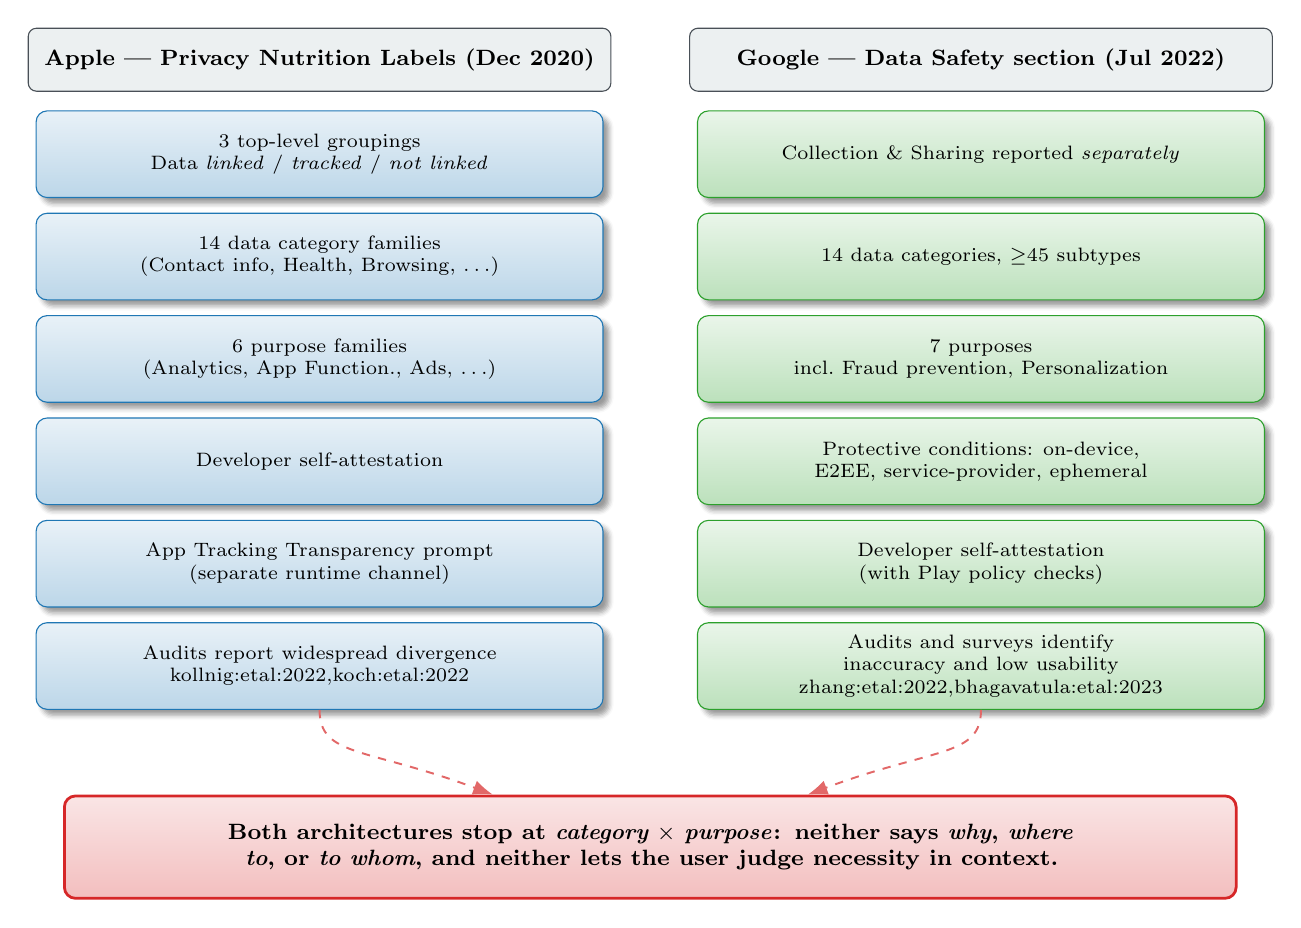
\begin{tikzpicture}[
    font=\sffamily,
    apple/.style={draw=ngBlue, top color=ngBlue!10, bottom color=ngBlue!30,
                  rounded corners=4pt, align=center, minimum width=72mm,
                  minimum height=11mm, font=\scriptsize,
                  blur shadow={shadow blur steps=4}},
    google/.style={draw=ngGreen, top color=ngGreen!10, bottom color=ngGreen!32,
                  rounded corners=4pt, align=center, minimum width=72mm,
                  minimum height=11mm, font=\scriptsize,
                  blur shadow={shadow blur steps=4}},
    header/.style={font=\bfseries\footnotesize, draw=ngSlate, fill=tierBg,
                   rounded corners=3pt, minimum width=74mm, minimum height=8mm},
    arr/.style={-{Latex[length=2.5mm]}, line width=0.7pt, draw=ngSlate}
]
\node[header] (HA) at (-4.2,7.6)  {Apple --- Privacy Nutrition Labels (Dec 2020)};
\node[header] (HG) at ( 4.2,7.6)  {Google --- Data Safety section (Jul 2022)};

\node[apple]  (a1) at (-4.2,6.4)  {3 top-level groupings\\Data \emph{linked} / \emph{tracked} / \emph{not linked}};
\node[apple]  (a2) at (-4.2,5.1)  {14 data category families\\(Contact info, Health, Browsing, $\ldots$)};
\node[apple]  (a3) at (-4.2,3.8)  {6 purpose families\\(Analytics, App Function., Ads, $\ldots$)};
\node[apple]  (a4) at (-4.2,2.5)  {Developer self-attestation};
\node[apple]  (a5) at (-4.2,1.2)  {App Tracking Transparency prompt\\(separate runtime channel)};
\node[apple]  (a6) at (-4.2,-0.1) {Audits report widespread divergence\\\citep{kollnig:etal:2022,koch:etal:2022}};

\node[google] (g1) at ( 4.2,6.4)  {Collection \& Sharing reported \emph{separately}};
\node[google] (g2) at ( 4.2,5.1)  {14 data categories, $\ge$45 subtypes};
\node[google] (g3) at ( 4.2,3.8)  {7 purposes\\incl.\ Fraud prevention, Personalization};
\node[google] (g4) at ( 4.2,2.5)  {Protective conditions: on-device,\\E2EE, service-provider, ephemeral};
\node[google] (g5) at ( 4.2,1.2)  {Developer self-attestation\\(with Play policy checks)};
\node[google] (g6) at ( 4.2,-0.1) {Audits and surveys identify\\inaccuracy and low usability\\\citep{zhang:etal:2022,bhagavatula:etal:2023}};

% Shared problem banner, placed with enough vertical clearance so the
% dashed connectors land on the banner's top edge rather than crowding
% the audit-row boxes above.
\node[draw=ngRed, line width=1pt, rounded corners=4pt,
      top color=ngRed!12, bottom color=ngRed!30,
      text width=14.6cm, minimum height=13mm,
      align=center, font=\bfseries\footnotesize, inner sep=4pt] at (0,-2.4) (banner)
    {Both architectures stop at \emph{category $\times$ purpose}: neither says
     \emph{why}, \emph{where to}, or \emph{to whom}, and neither lets the user
     judge necessity in context.};

% Dashed converging arrows from each audit-row to the banner.  Use
% Bezier curves so the lines arc inward gently and arrive at the banner
% top with clear margin from the boxes above.
\draw[arr, dashed, draw=ngRed!70]
   (a6.south) .. controls +(0,-0.6) and +(-1.6,0.6) .. (banner.north -| -2,0);
\draw[arr, dashed, draw=ngRed!70]
   (g6.south) .. controls +(0,-0.6) and +( 1.6,0.6) .. (banner.north -|  2,0);

\end{tikzpicture}%
}
\caption{Apple's Privacy Nutrition Labels and Google Play's Data Safety
section share the same category $\times$ purpose architecture. Both stop short
of the contextual information our results show users need.}
\label{fig:apple-vs-google}
\end{figure*}

The notice-and-choice model that underpins these labels rests on a strong
assumption: that category-level and purpose-level disclosure equips users
to judge an app's data practices
\citep{solove:2013,mcdonald:cranor:2008,cranor:2012}. The broader privacy
literature has long questioned that assumption on grounds of cognitive
cost, asymmetric information, and the well-documented gap between stated
preferences and behaviour in context~\citep{acquisti:etal:2015,
acquisti:etal:2017,acquisti:grossklags:2005,brandimarte:etal:2013}. For
app-store labels specifically, two failure modes are now documented.
Audits of both Apple and Google labels report systematic discrepancies
between declared and observed data practices~\citep{kollnig:etal:2022,
koch:etal:2022,bhagavatula:etal:2023}; user studies report low
comprehension of platform terminology and category
definitions~\citep{kelley:etal:2010,zhang:etal:2022,reidenberg:etal:2015}.
What is less understood is a third failure mode: \emph{judgment quality}.
How do users decide not merely whether data is collected or shared, but
whether a particular practice is \emph{necessary} given what the app is
for? The data-minimisation principle that underwrites both the European
Union's General Data Protection Regulation and post-GDPR proportionality
doctrine~\citep{gdpr:2016} requires personal data be ``adequate, relevant
and limited to what is necessary''; that necessity test, however, is
expected to be enforced from the user side only when the user can
exercise it.

This paper addresses the necessity-judgment question. We analyse two
existing data sources from a study of 87 Android micro-workers. The first
is a conceptual survey of mental models~\citep{wash:2010,lin:etal:2012,
kang:etal:2015}: which of the 14 Data Safety categories users regard as
personal, which of seven data-use purposes they regard as essential, and
how they interpret nine platform-defined boundary cases for collection and
sharing. The second is a task-based necessity evaluation in which the
same participants rated, on a five-point scale, whether collection and
sharing practices were necessary across 310 social apps drawn from
Google Play, and indicated whether the app description mentioned those
practices. The participant-level linkage between the two files is the
methodological keystone: it lets us ask whether the same person's
\emph{abstract} category beliefs predict their \emph{concrete}
app-specific necessity judgments.

The data surface several connected observations. First, users do not regard Data Safety
categories as uniformly personal: classification rates range from 42.5\,\%
(calendar) to 78.2\,\% (personal information). Second, users are uncertain
about policy boundary cases; in particular, fewer than half agree that
off-device ephemeral processing is non-collection or that
service-provider transfer is non-sharing. Third, task-level necessity
ratings sit near the scale midpoint
($M_{\text{coll}}=3.17$, $M_{\text{share}}=3.27$), with roughly a quarter
of all ratings neutral. Fourth, description-level mention of data
practices is not associated with higher perceived necessity; for sharing
practices the mention group is associated with \emph{lower} ratings than
the non-mention group. Fifth, the participant-level linkage shows that
classifying a category as personal predicts only slightly lower necessity
ratings for collection and no consistent difference for sharing;
cluster-bootstrap confidence intervals include zero in both directions.

We describe this between-tier pattern as the \emph{Necessity Gap}: a
descriptive label for the absence, in our data, of a detectable link
between category-level personalness judgments and the contextual
necessity judgments people make about specific app practices.
``Descriptive'' is meant strictly: the present design is observational
and the central RQ5 interval ($\pm 0.45$) does not allow us to
distinguish a within-person disconnect from a small effect we are
unable to detect at $N=87$. The notion is useful as an organising
device because category-level recognition, boundary acceptance and
contextual necessity behave differently in our data, and because the
exercise of articulating that difference points to the kinds of
information --- recipient, feature, alternative --- that current
labels do not carry. A user may rate location as deeply personal yet
see a navigation app's use of it as necessary; the same user may rate
calendar data as ambiguous yet object to a social game requesting it
without explanation. Neither the personalness judgment nor the
category-level disclosure alone settles the question. We treat the
three-tier architecture (Figure~\ref{fig:necessity-gap-architecture})
as a framework hypothesis to be evaluated in future, adequately
powered work, not as a finding established by the present study.

\begin{figure*}[!tbp]
\centering
\resizebox{\linewidth}{!}{%
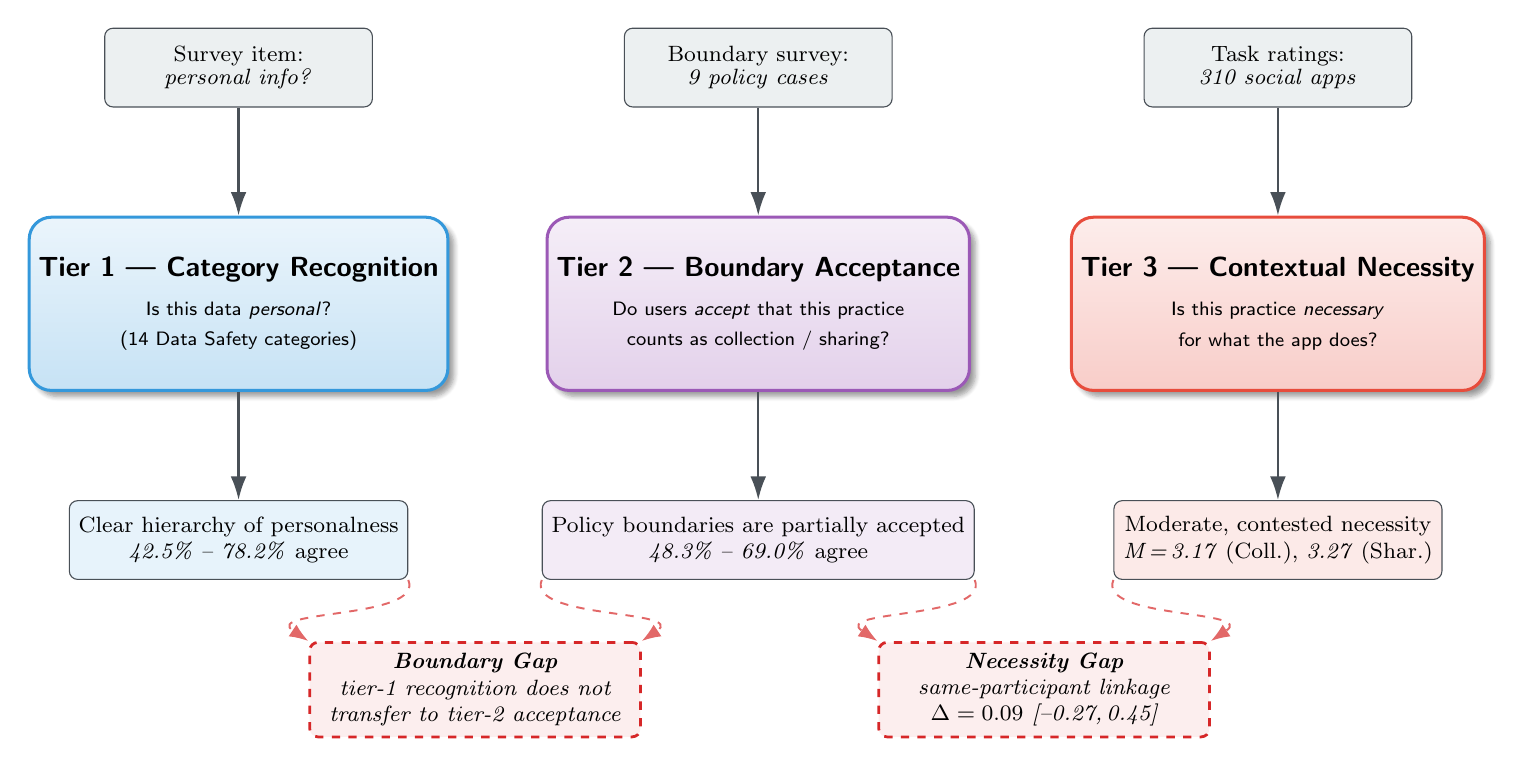
\begin{tikzpicture}[
    font=\sffamily,
    every node/.style={transform shape},
    tier/.style    = {rounded corners=8pt, draw=#1, line width=1.1pt,
                      top color=#1!10, bottom color=#1!28,
                      minimum width=46mm, minimum height=22mm,
                      align=center, blur shadow={shadow blur steps=6}},
    inputbox/.style= {draw=ngSlate, rounded corners=3pt, fill=tierBg,
                      align=center, minimum width=34mm, minimum height=10mm,
                      font=\footnotesize},
    gap/.style     = {draw=ngRed, rounded corners=3pt, dashed, line width=1.0pt,
                      fill=ngRed!8, align=center, font=\footnotesize\itshape,
                      minimum width=42mm, minimum height=12mm},
    flow/.style    = {-{Latex[length=3mm,width=2mm]}, line width=0.9pt,
                      draw=ngSlate},
    gapflow/.style = {-{Latex[length=2.4mm,width=1.8mm]}, line width=0.7pt,
                      draw=ngRed!70, dashed}
]

% Tier nodes (the three judgment levels)
\node[tier=tierA] (T1) at (0,4) {%
    \textbf{Tier 1 --- Category Recognition}\\[2pt]
    \scriptsize Is this data \emph{personal}?\\[-1pt]
    \scriptsize (14 Data Safety categories)
};
\node[tier=tierB] (T2) at (6.6,4) {%
    \textbf{Tier 2 --- Boundary Acceptance}\\[2pt]
    \scriptsize Do users \emph{accept} that this practice\\[-1pt]
    \scriptsize counts as collection / sharing?
};
\node[tier=tierC] (T3) at (13.2,4) {%
    \textbf{Tier 3 --- Contextual Necessity}\\[2pt]
    \scriptsize Is this practice \emph{necessary}\\[-1pt]
    \scriptsize for what the app does?
};

% Inputs above each tier
\node[inputbox] at (T1 |- 0,7.0) (i1) {Survey item:\\[-1pt]\emph{personal info?}};
\node[inputbox] at (T2 |- 0,7.0) (i2) {Boundary survey:\\[-1pt]\emph{9 policy cases}};
\node[inputbox] at (T3 |- 0,7.0) (i3) {Task ratings:\\[-1pt]\emph{310 social apps}};

\draw[flow] (i1) -- (T1);
\draw[flow] (i2) -- (T2);
\draw[flow] (i3) -- (T3);

% Results below each tier (with their headline numbers)
\node[inputbox, fill=tierA!12] at (T1 |- 0,1.0) (r1)
    {Clear hierarchy of personalness\\
     \emph{42.5\% \textendash{} 78.2\%} agree};
\node[inputbox, fill=tierB!12] at (T2 |- 0,1.0) (r2)
    {Policy boundaries are partially accepted\\
     \emph{48.3\% \textendash{} 69.0\%} agree};
\node[inputbox, fill=tierC!12] at (T3 |- 0,1.0) (r3)
    {Moderate, contested necessity\\
     \emph{M\,=\,3.17} (Coll.), \emph{3.27} (Shar.)};

\draw[flow] (T1) -- (r1);
\draw[flow] (T2) -- (r2);
\draw[flow] (T3) -- (r3);

% Between-tier "gap" annotations.  Routing: each gap node sits lower than
% the result row so the connecting dashed arrows have visible clearance
% from the result boxes (rather than touching their edges).
\node[gap] at ($(r1.east)!0.5!(r2.west) + (0,-1.9)$) (G12) {%
    \textbf{Boundary Gap}\\
    tier-1 recognition does not\\transfer to tier-2 acceptance};
\node[gap] at ($(r2.east)!0.5!(r3.west) + (0,-1.9)$) (G23) {%
    \textbf{Necessity Gap}\\
    same-participant linkage\\$\Delta=0.09$ [\textendash 0.27,\,0.45]};

% Smooth dashed connectors that leave the result boxes on the side rather
% than from the bottom centre; this keeps the arrowheads from overlapping
% the gap-box borders.
\draw[gapflow] (r1.south east) .. controls +(0.2,-0.5) and +(-0.6,0.4) .. (G12.north west);
\draw[gapflow] (r2.south west) .. controls +(-0.2,-0.5) and +( 0.6,0.4) .. (G12.north east);
\draw[gapflow] (r2.south east) .. controls +(0.2,-0.5) and +(-0.6,0.4) .. (G23.north west);
\draw[gapflow] (r3.south west) .. controls +(-0.2,-0.5) and +( 0.6,0.4) .. (G23.north east);

\end{tikzpicture}%
}
\caption{Three-tier conceptual architecture of the Necessity Gap. Each
tier draws on a distinct empirical source in the present study. The
Boundary Gap and the Necessity Gap describe the two between-tier
breakdowns observed in the data and are presented as a framework
hypothesis rather than as confirmed within-person disconnects.}
\label{fig:necessity-gap-architecture}
\end{figure*}


The paper contributes the following. First, empirically, we provide
an exploratory, participant-level characterisation of how Android
users interpret and judge Google Play Data Safety disclosures, with
documented validation of data artefacts, robustness checks across
six response-quality filters, a precision analysis bounding what
RQ5 can detect at $N=87$, and a category $\times$ purpose
\emph{evidence-density map} of the practices users encountered in the
310-app corpus (4{,}368 collection and 994 sharing app-practice
instances). Second, conceptually, we introduce the \emph{Necessity
Gap} as a descriptive framework for organising results across three
tiers --- category recognition, boundary acceptance, contextual
necessity --- and connect that framework to Nissenbaum's
contextual-integrity
theory~\citep{nissenbaum:2004,nissenbaum:2010,barth:etal:2006},
Solove's consent dilemma~\citep{solove:2013}, and the GDPR's
proportionality principle~\citep{gdpr:2016}. We propose the
three-tier architecture (Figure~\ref{fig:three-tier-flow}) as a
working hypothesis for the design and evaluation of contextual
disclosures rather than as an empirical finding of the present study.
Third, on the design side, we offer five \emph{proposed design
implications} --- \emph{Why--Where--Who--Control--Flag} (WWWCF) ---
that point to the parts of the existing label architecture where our
data identify the largest evidence gaps (Figure~\ref{fig:wwwcf-radial}),
together with an illustrative worked redesign sketch
(Figure~\ref{fig:mockup-redesign}). The design implications are
explicitly motivated by, not validated against, the present data.
Fourth, we propose --- and explicitly leave to future empirical
validation, with no rubric instantiation or inter-coder reliability
reported in this paper --- that the same five-question structure
might be repurposed as an evaluation rubric:
instead of judging labels by trust or install intention, future
studies could measure whether users can articulate the relationships
among data type, app function, recipient, processing boundary, and
available control. We mark the rubric proposal as a hypothesis rather
than a finished instrument; the empirical evaluation of a WWWCF-built
label remains future work.

Section~\ref{sec:related-work} reviews privacy labels, notice-based
design, mental-model research, contextual integrity, audits of mobile
privacy, and disclosure evaluation.
Section~\ref{sec:research-questions} states the five research questions.
Section~\ref{sec:method} describes data sources, validation procedures,
linkage strategy, statistical approach, and the quality-aware analysis
strategy. Section~\ref{sec:results} reports RQ1--RQ5 with colourful
figures derived from the raw data and adds a category $\times$ purpose
evidence map and a qualitative analysis of free-text rationales.
Section~\ref{sec:necessity-gap} develops the Necessity Gap construct.
Section~\ref{sec:design} develops the WWWCF design requirements and a
worked label redesign. Section~\ref{sec:evaluation-metrics} proposes a
a candidate evaluation rubric. Section~\ref{sec:limitations} discusses
limitations and threats to validity. Section~\ref{sec:future} lists
planned follow-up studies, and Section~\ref{sec:ethics} reports ethics,
compensation details, and data availability. Section~\ref{sec:conclusion}
concludes.

%==========================================================================
\section{Related Work}
\label{sec:related-work}

The paper sits at the intersection of five literatures: privacy
disclosure design, mental models of mobile privacy, contextual integrity
and the proportionality principle, audits of app-store labels, and
disclosure evaluation methodology. We summarise each in turn.

\subsection{App-Store Privacy Labels and Disclosures}
\label{subsec:rw-labels}

Privacy labels for software have been studied for more than a
decade.~\citet{kelley:etal:2009,kelley:etal:2010} designed a standardised
``privacy nutrition label'' for websites and showed that structured,
at-a-glance presentation improved comprehension and the accuracy of
privacy-informed choices compared with policy
prose.~\citet{kelley:etal:2013} extended the framework to mobile app
selection and demonstrated that users incorporated label information
into install decisions when it was made visible at the right
time.~\citet{schaub:etal:2015} mapped the design space for privacy
notices on mobile, identifying timing, channel, modality, and content
framing as critical, and~\citet{egelman:etal:2009} showed that the
timing of privacy indicators (before vs.\ during purchase) materially
affects user behaviour. These efforts informed two platform deployments:
Apple's App Store Privacy Nutrition Labels (December 2020) and Google
Play's Data Safety section (July 2022). Both adopt category-based
architectures: Apple uses three top-level groupings (data linked to
identity, data used to track, data not linked) over 14 category families
and 6 purposes; Google uses 14 data-category families covering
$\geq$\,45 subtypes, 7 purposes, and reports collection and sharing
separately, with attestations for protective conditions
(Figure~\ref{fig:apple-vs-google}).

Early empirical evaluations of these labels identify accuracy and
comprehension problems.~\citet{kollnig:etal:2022} find widespread
divergence between Apple label claims and observed tracking behaviour
using network monitoring;~\citet{koch:etal:2022} audit label content
against privacy policies and document systematic inaccuracies and
inconsistent terminology;~\citet{zhang:etal:2022} show that Apple's
labels suffer from confusing structure, unfamiliar terminology, and
disconnection from in-app controls, with many participants unaware they
exist.~\citet{bhagavatula:etal:2023} interview developers about how
they fill in Privacy Nutrition Labels and report a third problem: even
when developers want to comply, the categories and instructions are
ambiguous from the producer side, producing inconsistent declarations
across apps that ostensibly process the same data. Our study adds a
fourth layer to this picture by asking whether users can form
\emph{necessity judgments} on the disclosed practices, given that they
have noticed and nominally understand the labels.

\subsection{Limitations of Notice-Based Privacy Design}
\label{subsec:rw-notice}

Notice-and-choice has been challenged structurally and
empirically.~\citet{solove:2013} argues the model cannot scale to modern
data environments: the cost and complexity of evaluating every
disclosure exceed realistic user capacity.~\citet{mcdonald:cranor:2008}
estimate that a U.S. internet user attempting to read every privacy
policy they encountered annually would need approximately 76 work days,
at a national opportunity cost in the order of \$781 billion. Standardised
labels reduce reading burden but also reduce information: a category
label such as ``Location'' conveys less than a prose passage describing
when, how, and to whom location data flows~\citep{cranor:2012}.
\citet{acquisti:etal:2015,acquisti:etal:2017,acquisti:grossklags:2005}
show that privacy decisions are highly sensitive to framing, defaults,
and context, in ways that depart from rational utility
maximisation.~\citet{brandimarte:etal:2013} show that increasing apparent
control over disclosure can paradoxically increase risky disclosure ---
the so-called \emph{control paradox}.~\citet{jensen:potts:2004} compared
privacy policies and shorter notices and concluded that condensed
notices were necessary but not sufficient for informed
decisions.~\citet{tsai:etal:2011} demonstrated experimentally that
privacy information presented prominently at the point of purchase
shifted online buyer behaviour. Together, this work implies that
disclosure format, not only presence, decides whether users can act.

In the Android setting,~\citet{felt:etal:2012} documented this problem
at the permission layer: many users granted permissions without reading
them, and among those who did, comprehension of scope was
low.~\citet{felt:etal:2012b} surveyed concerns and found that users were
worried about specific feature consequences (e.g., reading SMS, taking
pictures) rather than about permissions in the
abstract.~\citet{tan:etal:2014} showed that developer-supplied
explanations for permission requests substantially increased grant rates,
indicating that contextual rationales are influential when
present.~\citet{liccardi:etal:2014} demonstrated that augmenting app
selection with sensitivity scores helped non-technical users select
apps with lower data exposure. The failure was not that users ignored
notices, but that the permission names did not contextualise
\emph{why} the access was needed for a specific app. Data Safety labels
face an analogous challenge: category and purpose names are defined by
platform policy, not by the features users interact with.

\subsection{User Mental Models of Mobile Data Practices}
\label{subsec:rw-mental-models}

Research on mental models of data collection has consistently found that
users reason about privacy through context, purpose, and perceived
benefit rather than category alone~\citep{lin:etal:2012,lin:etal:2014,
ur:etal:2012,kang:etal:2015}.~\citet{lin:etal:2012} used a crowdsourced design to show
that expectation accuracy varies with app function: users expect a
mapping app to use location but are surprised when a game does.
\citet{lin:etal:2014} extended this line of work into a clustering of
users' mobile-app privacy preferences, demonstrating that personalised
default settings derived from a small number of preference profiles
can sharply reduce the number of explicit permission decisions users
must make.~\citet{ur:etal:2012} find that reactions to behavioural
advertising range from comfort to alarm depending on what data is used
and for what.~\citet{kang:etal:2015} interviewed users and found a wide
range of folk theories of how data moves between sites and apps:
``my data just goes everywhere'' was a common
trope.~\citet{wash:2010,wash:rader:2015} show that folk models of
computer security determine which protective actions people take, and
that more technical knowledge does not always produce more protective
behaviour. A related pattern may apply to privacy labels: users may rely
on categorical heuristics (\emph{``financial data is always sensitive''},
\emph{``app performance data is harmless''}) that do not align with the
privacy implications of specific practices. The participant-linked
analysis we develop in Section~\ref{sec:results} tests this directly.

The classical privacy theorists of the twentieth century already
anticipated these contextual dynamics.~\citet{westin:1967} defined
privacy as the claim of individuals to determine for themselves when,
how, and to what extent information about them is communicated to
others, foregrounding agency.~\citet{altman:1975} reframed privacy as a
dynamic, dialectical regulation of boundaries between self and others,
and~\citet{petronio:2002} extended this into a theory of communication
privacy management built around boundary co-ownership and disclosure
rules. The platform-side question is whether category $\times$ purpose
labels give users enough information to operate as privacy boundary
managers in the sense of these theories. Our results suggest they do not.

\subsection{Contextual Integrity and Proportionality}
\label{subsec:rw-contextual-integrity}

Nissenbaum's contextual integrity (CI) framework~\citep{nissenbaum:2004,
nissenbaum:2010} provides the most developed theoretical account of why
category-level disclosure is insufficient: privacy norms are not defined
by data sensitivity in the abstract but by the appropriateness of
information flows relative to the norms of a social
context.~\citet{barth:etal:2006} formalised CI as a logic of information
flows for compliance reasoning. CI has since been operationalised in
empirical work on smart-home devices~\citep{apthorpe:etal:2018}, mobile
permissions~\citep{wijesekera:etal:2015,wijesekera:etal:2017},
privacy-policy text~\citep{shvartzshnaider:etal:2019}, and on the
relationship between context and confounding
variables~\citep{martin:nissenbaum:2017}. A Data Safety label that names
a category and a purpose provides only partial contextual information; it
omits recipient, processing boundary, retention, and the specific app
feature that makes the practice necessary --- four of the five CI
parameters (actor, attribute, transmission principle, context).

The concept of data necessity operationalises a related requirement in
regulation. The GDPR's data-minimisation principle requires personal data
be ``adequate, relevant and limited to what is necessary''
\citep{gdpr:2016}. For this to be enforceable from the user side, users
must be able to judge whether a practice is proportionate. Our study
examines whether the information structure of Data Safety labels
supports such judgments. The complementary research programme of
``privacy by design''~\citep{spiekermann:cranor:2009,cavoukian:2009}
proposes that data-minimisation be engineered into systems rather than
left to user inspection, but a user-facing necessity test remains a
required component for any post-hoc accountability regime.

\subsection{Mobile Privacy Audits and Disclosure Quality}
\label{subsec:rw-audits}

A line of measurement work has examined whether mobile apps actually do
what their notices claim. Network-level monitoring of Android apps
\citep{englehardt:narayanan:2016,razaghpanah:etal:2018,ren:etal:2018}
documents pervasive use of third-party analytics and advertising SDKs
that exfiltrate device identifiers and behavioural traces.
~\citet{reyes:etal:2018} measured COPPA non-compliance at scale in
children's apps.~\citet{andow:etal:2020} introduced \textsc{PoliCheck},
which compares stated privacy policy claims to observed data flows at
the granularity of the recipient party and reports systematic mismatches.
~\citet{kollnig:etal:2022} and~\citet{koch:etal:2022} extend this work
to the era of formal app-store labels and identify a recurring pattern:
many declared labels are technically defensible under the relevant
platform policy yet do not communicate the practice in a user-meaningful
way. This audit literature shows that even when labels are filled in
correctly, the categories and exceptions in the label are themselves
opaque; our study completes the loop by showing that the opacity blocks
necessity judgment at the user side.

\subsection{Evaluation of Privacy Disclosure Comprehension}
\label{subsec:rw-evaluation}

Most evaluations of privacy disclosures measure whether users can
\emph{recall} or identify disclosed
facts~\citep{kelley:etal:2010,zhang:etal:2022,reidenberg:etal:2015}.
Judgment quality is a distinct construct: a user may correctly recall
that an app collects location while still failing to judge whether that
collection is proportionate to the app's function. Several recent
studies have moved towards behaviourally meaningful
metrics.~\citet{almuhimedi:etal:2015} used permission ``nudges'' that
displayed cumulative usage counts (e.g., ``Your location has been shared
5{,}398 times'') and observed that users revoked permissions when given
this contextual information.~\citet{naeini:etal:2017} measured
information-flow expectations in the IoT setting and showed that
acceptance was sharply context-dependent.~\citet{habib:etal:2020} found
that even when websites provide opt-out and deletion options as required
by recent regulations, the controls are difficult to find and use,
suggesting that the burden of necessity judgment is compounded by a
control-discovery burden.~\citet{wijesekera:etal:2017} used contextual
prompts to dynamically grant Android permissions in a way that aligned
better with users' preferences than the static permission model. Our
study uses a task-based necessity rating design rather than a recall
task, measuring judgment quality directly. We additionally link
survey-level attitude data to task-level ratings at the participant
level, which lets us characterise the Necessity Gap as a
within-participant pattern rather than an aggregate between-sample
contrast.

The recent work by~\citet{wilson:etal:2016} on the OPP-115 privacy
policy corpus has stimulated automated analyses of disclosure text;
work by~\citet{balebako:etal:2014} demonstrated that visualising data
leaks raised user awareness even when the underlying flows were already
disclosed in policies.~\citet{egelman:etal:2013} showed that even when
users would in principle pay for less data-hungry apps, the choice
architecture of app stores often made the comparison difficult. Our
findings extend this line of work to the post-label era: making practices
visible at the level of categories and purposes is necessary but not
sufficient~\citep{cranor:2012}.

%==========================================================================
\section{Research Questions}
\label{sec:research-questions}

Guided by the gap between category-level disclosure and contextual
necessity judgment, we ask five research questions.

\begin{description}
    \item[\bfseries RQ1.] Which Google Play Data Safety categories do
    users classify as personal, non-personal, or ambiguous, and how flat
    or graded is the resulting category map?
    \item[\bfseries RQ2.] How do users interpret the nine
    platform-defined collection and sharing boundary cases (off-device
    ephemeral processing, service-provider transfer, consent,
    anonymisation, on-device-only, end-to-end encryption, redirect to
    service, legal transfer, and user-initiated transfer)?
    \item[\bfseries RQ3.] How necessary do users judge collection and
    sharing practices in app-level tasks over a 310-app corpus, and how
    does necessity vary by data category and use purpose?
    \item[\bfseries RQ4.] Is description-level mention of data practices
    associated with higher perceived necessity?
    \item[\bfseries RQ5.] Within the same participants, does classifying
    a data category as personal predict judging app practices involving
    that category as less necessary?
\end{description}

These questions are intentionally non-causal. The empirical target is the
\emph{current} relationship among users' mental models, app-description
disclosure, and necessity judgments under Google Play's existing label
architecture. We complement RQ1--RQ5 with a category $\times$ purpose
evidence map (Section~\ref{subsec:cat-purpose-map}) and a qualitative
audit of free-text rationales (Section~\ref{subsec:qualitative}) that
together triangulate the quantitative pattern.

%==========================================================================
\section{Method}
\label{sec:method}

\subsection{Participants and Recruitment}
\label{subsec:participants}

Eighty-seven Android users were recruited from the Microworkers
crowd-work platform between February and April 2024. Microworkers is a
long-running paid task platform with documented use in HCI studies
(crowd recruitment is also used for related work by
\citealt{lin:etal:2012,naeini:etal:2017}). Recruitment screened for
self-reported active Android use, English literacy sufficient to read
Google Play app descriptions, and a Microworkers job-success rate of
$\geq 85$\,\%. The expected task time was 30 minutes for the combined
survey-plus-assessment instrument; participants were paid USD\,2.00
per completed task, plus a USD\,0.50 bonus for completing both
instruments in a single session, consistent with the platform's
recommended fair-pay benchmark and the regional cost-of-living
adjustment Microworkers applies to its task rates. The study was
approved by the host institution's human research ethics committee
(approval reference anonymised for review); the consent form disclosed
that responses and email addresses would be used for non-commercial
research, that emails would serve only as join keys and would be
discarded from analysis outputs, and that participants could withdraw
without penalty. Of the 87 participants, 70 completed both
instruments; the remaining 17 contributed survey responses only and
appear in the survey-side analyses but not in the task-side ones.
Demographic items (age, gender, education, country of residence) were
collected but are not reported below in detail because the cell sizes
are too small to support per-group analysis and we did not pre-register
demographic hypotheses.

\subsection{Survey Instrument}
\label{subsec:survey}

The \emph{conceptual survey} (33 columns, 30 substantive items)
elicited:
(i) \emph{personalness} judgments for the 14 Data Safety categories
(Location, Personal info, Financial info, Health and fitness, Messages,
Photos and videos, Audio files, Files and docs, Calendar, Contacts, App
activity, Web browsing, App info and performance, Device or other IDs);
(ii) \emph{essentiality} judgments for seven Data Safety purposes
(Account management, Advertising or marketing, App functionality,
Analytics, Developer communications, Fraud prevention/security/compliance,
Personalization); and
(iii) Yes/No/Maybe responses to nine policy boundary cases drawn from
the Google Play Data Safety policy text (Section~\ref{subsec:rq2-boundaries}
lists the exact items). Each item was followed by a short free-text
rationale; the corpus contains 2{,}610 such rationales.

\subsection{Task-Based Necessity Assessment}
\label{subsec:task}

The \emph{task-based assessment} (615 columns) presented a series of
real Google Play social-app descriptions. For each assigned app,
participants:
(i) read the app description as it appeared on the store;
(ii) indicated whether the description \emph{mentioned} collection and
sharing of data;
(iii) selected the Data Safety categories the app declared as collected
and shared;
(iv) for each collected/shared category, selected the purpose(s) the
app declared;
(v) for each (category, purpose) instance, provided a five-point
necessity rating, anchored at 1\,=\,Very unnecessary and 5\,=\,Very
necessary.

The task corpus contains 310 distinct social apps (309 unique English
or transliterated names), drawn from English- and non-English-language
markets to reflect the international composition of Google Play
\citep{kollnig:etal:2022,bhagavatula:etal:2023}. After validation
(Section~\ref{subsec:data-validation}), the usable analytic dataset
consists of 1{,}690 collection ratings from 82 participants and 661
sharing ratings from 75 participants. The Analysis sub-corpus contains
4{,}368 collection plus 994 sharing distinct app-practice instances
(5{,}362 in total) over the 13 of the 14 Data Safety categories that
received non-zero practice evidence in the corpus (the 14th, Audio
files, was rated as personal by 50.6\,\% of participants in the
survey but received zero task-level evidence in the 310-app corpus
and is therefore absent from the evidence map though present in the
personalness analysis). The 13 categories with non-zero evidence are
App activity, App info/perf., Calendar, Contacts, Device IDs,
Files/docs, Financial info, Health/fit., Location, Messages, Personal
info, Photos/videos, and Web browsing. The seven Google Play purposes
(Account management, Advertising or marketing, App functionality,
Analytics, Developer communications, Fraud prevention/security/compliance,
Personalization) appear as the column dimension.

\subsection{Aggregate App-Level File}
\label{subsec:app-level}

We additionally use \texttt{app-selection(percent).csv} (310 rows of
app-level aggregate agreement/disagreement, one row per app) for
descriptive app-level summaries only. This file aggregates over
participants and is the only source of app identity at this level: it
records, for each app, the share of participants who rated the app's
reported practices as necessary, but it does \emph{not} carry the
per-participant rating for each app. The user-level task ratings file
(\texttt{user-selection.csv}) does carry per-participant rating events,
indexed by participant and by category/practice, which supports the
participant-cluster bootstrap used for RQ5; the app identifier in that
file is, however, encoded only as a position in a participant's task
queue rather than as a stable global app key, so cross-app
random-effects modelling at the rating level cannot be reconstructed
from the present export without re-keying. We mark a re-keyed
mixed-effects re-analysis as part of the planned follow-up
(Section~\ref{sec:future}).

\paragraph{Data provenance.} Table~\ref{tab:provenance} maps every
reported $N$ to its raw source so the path from raw file to derived
variable is explicit.

\begin{table}[t]
\centering
\caption{Data provenance: every $N$ reported in the paper traced to
its raw source file, derived variable, and the figure or table where
it appears. ``Necessity rating'' refers to the five-point category
necessity rating that is usable for analysis; the (category, purpose)
rating column is the export-defective field and is not used as a
rating (see Section~\ref{subsec:data-validation}).}
\label{tab:provenance}
\small
\begin{tabular}{p{0.20\linewidth}p{0.30\linewidth}p{0.10\linewidth}p{0.30\linewidth}}
\toprule
\textbf{Raw source} & \textbf{Derived variable / unit} & \textbf{$N$}
                   & \textbf{Figure / table} \\
\midrule
\texttt{survey-stats.csv}
  & Personalness, Y/N/M per category $\times$ participant
  & 87 part.\ $\times$ 14 cat.
  & Fig.~\ref{fig:rq1-personalness}; RQ1 \\
\texttt{survey-stats.csv}
  & Boundary acceptance, Y/N/M per case $\times$ participant
  & 87 part.\ $\times$ 9 cases
  & Fig.~\ref{fig:rq2-boundaries}; Fig.~\ref{fig:boundary-tree}; RQ2 \\
\texttt{user-selection.csv}
  & Category-level necessity rating (1--5) per (participant, app, category)
  & 1{,}690 coll., 661 shar.
  & Fig.~\ref{fig:rq3-necessity-stacked};
    Table~\ref{tab:category-necessity}; RQ3, RQ4 \\
\texttt{user-selection.csv}
  & Description-mention flag per (participant, app)
  & 70 part.; 310 apps
  & Fig.~\ref{fig:rq4-description-mention}; RQ4 \\
\texttt{user-selection.csv} $\bowtie$ \texttt{survey-stats.csv}
  & RQ5 linkage: $\bar{N}_{ica}$ per (participant, category, action)
  & 2{,}323 rat.\ obs., 1{,}080 part.-cat.\ obs.
  & Fig.~\ref{fig:rq5-necessity-gap}; Table~\ref{tab:rq5-linkage}; RQ5 \\
\texttt{Analysis/*\_P.csv}
  & Evidence-density indicator and parsed ``$k$ apps'' count per
    (participant, category, purpose)
  & 4{,}368 coll., 994 shar.
  & Figs.~\ref{fig:heatmap-coll}, \ref{fig:heatmap-shar};
    Tables \ref{tab:cat-evidence-coll}, \ref{tab:cat-evidence-shar} \\
\texttt{app-selection-}\par\texttt{(percent).csv}
  & App-level Agree $\%$: share of participants rating the app's
    reported practices $\geq 4$
  & 310 apps
  & Fig.~\ref{fig:app-level-agreement}; \S~\ref{subsec:app-level-agreement} \\
\bottomrule
\end{tabular}
\end{table}

\subsection{Analysis Architecture}
\label{subsec:analysis-architecture}

Figure~\ref{fig:analysis-architecture} summarises the pipeline. Raw
survey and task CSV files are authoritative; derived files are used
only for triangulation unless their values can be reproduced.
Participant emails are used only as internal join keys and are removed
from every reported output.

\begin{figure}[!htbp]
\centering
\resizebox{\linewidth}{!}{%
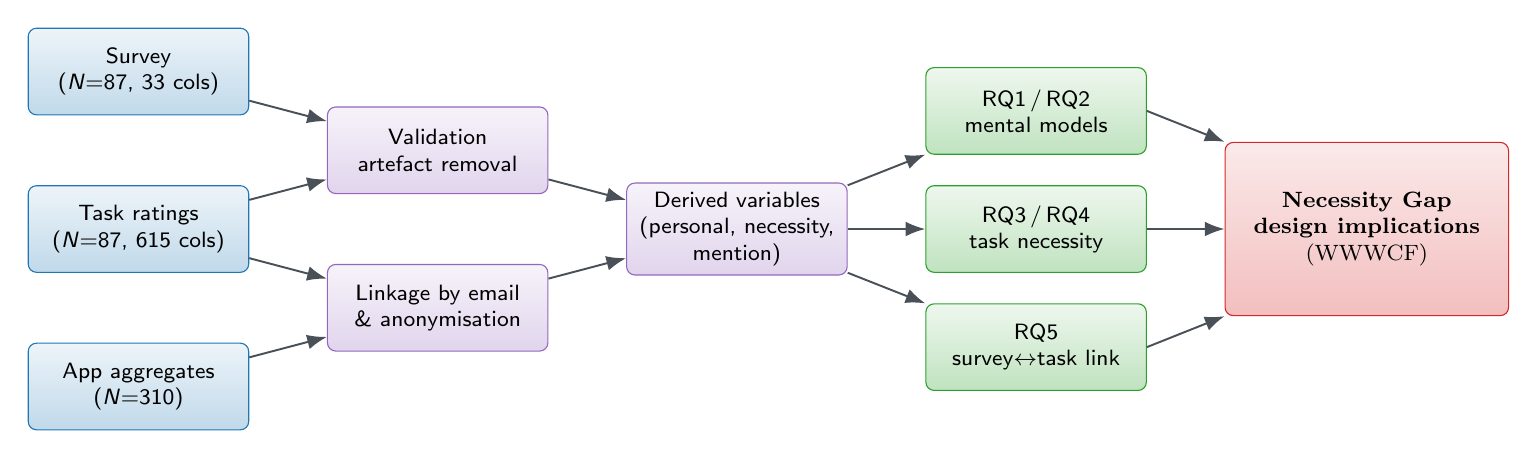
\begin{tikzpicture}[
    font=\sffamily\footnotesize, >=Latex,
    src/.style={draw=ngBlue, top color=ngBlue!8, bottom color=ngBlue!28,
                rounded corners=3pt, align=center, minimum width=28mm,
                minimum height=11mm},
    proc/.style={draw=ngPurple, top color=ngPurple!8, bottom color=ngPurple!28,
                rounded corners=3pt, align=center, minimum width=28mm,
                minimum height=11mm},
    result/.style={draw=ngGreen, top color=ngGreen!8, bottom color=ngGreen!30,
                rounded corners=3pt, align=center, minimum width=28mm,
                minimum height=11mm},
    impl/.style={draw=ngRed, top color=ngRed!10, bottom color=ngRed!30,
                rounded corners=3pt, align=center, minimum width=36mm,
                minimum height=22mm, font=\footnotesize},
    arr/.style={-{Latex[length=2.5mm]}, line width=0.7pt, draw=ngSlate}
]
% Left column: three raw data sources
\node[src] (s1) at (0,4) {Survey\\(\textit{N}=87, 33 cols)};
\node[src] (s2) at (0,2) {Task ratings\\(\textit{N}=87, 615 cols)};
\node[src] (s3) at (0,0) {App aggregates\\(\textit{N}=310)};

% Second column: validation and linkage processes
\node[proc] (p1) at (3.8,3) {Validation\\artefact removal};
\node[proc] (p2) at (3.8,1) {Linkage by email\\\& anonymisation};

% Third column: derived-variable hub
\node[proc] (p3) at (7.6,2) {Derived variables\\(personal, necessity,\\mention)};

% Fourth column: three RQ results
\node[result] (r1) at (11.4,3.5) {RQ1\,/\,RQ2\\mental models};
\node[result] (r2) at (11.4,2.0) {RQ3\,/\,RQ4\\task necessity};
\node[result] (r3) at (11.4,0.5) {RQ5\\survey$\leftrightarrow$task link};

% Fifth column: implications, placed to the RIGHT of the result column
% so each result connects with a single horizontal-ish arrow and the
% arrows do not cross one another.
\node[impl] (i1) at (15.6,2.0)
    {\textbf{Necessity Gap}\\\textbf{design implications}\\(WWWCF)};

% Source -> processing arrows.
\draw[arr] (s1) -- (p1);
\draw[arr] (s2) -- (p1);
\draw[arr] (s2) -- (p2);
\draw[arr] (s3) -- (p2);

% Processing -> derived-variable hub.
\draw[arr] (p1) -- (p3);
\draw[arr] (p2) -- (p3);

% Hub -> three RQ results.
\draw[arr] (p3) -- (r1);
\draw[arr] (p3) -- (r2);
\draw[arr] (p3) -- (r3);

% Results -> implications.  Three direct arrows from each result box's
% east edge to the implications box's west edge.  Because i1 sits to the
% right of the result column at the same vertical centre as r2, the
% three arrows fan in cleanly without crossing.
\draw[arr] (r1.east) -- (i1.north west);
\draw[arr] (r2.east) -- (i1.west);
\draw[arr] (r3.east) -- (i1.south west);

\end{tikzpicture}%
}
\caption{Analysis architecture. Raw survey and task files (left) feed
the validation and linkage stages, which produce derived variables
that are evaluated against the five research questions. The three RQ
findings converge into the Necessity-Gap design implications (right),
via three direct arrows that fan in from the result column without
crossing any other box.}
\label{fig:analysis-architecture}
\end{figure}


\subsection{Data Validation}
\label{subsec:data-validation}

We performed four validation checks before any analysis.

\textbf{Survey summary consistency.} The derived file
\texttt{survey-stat(percent).txt} reports 0\,\% for all No responses,
which contradicts the raw survey file. All survey percentages are
therefore computed from \texttt{survey-stats.csv} rather than the
derived summary.

\textbf{Participant linkage.} Both raw files contain 87 non-empty,
unique participant emails; all 87 match. The one-to-one match supports
the RQ5 linkage. Emails are dropped after the join.

\textbf{Purpose-rating artefact and salvage strategy.} All non-empty
values in the task file's collection-purpose ($n=3{,}670$) and
sharing-purpose ($n=842$) sections are coded as ``Very unnecessary''.
Inspection of the data-export pipeline indicates that the rating
column was populated from a constant default rather than from the
participant's rating control; the random variation that would be
present if the values reflected real responses is entirely absent
across all $4{,}512$ non-empty cells. We treat these values as
\emph{not interpretable as necessity ratings} and exclude the task
purpose ratings from the necessity analysis.

We do, however, retain two pieces of information that the artefact
does not destroy. (i) The \emph{evidence indicator}: whether a cell is
non-empty, i.e.\ whether the participant claimed the practice occurred
for that (app, category, purpose). (ii) The \emph{evidence count}: the
``$k$'' value in the ``Un($k$ apps)'' annotation that the export
appends to each non-empty cell. The evidence count is written into the
cell text by a different code path from the rating control: it is a
parse of the participant's earlier app-selection step, not a copy of
their five-point rating. Three diagnostics support that the indicator
and count are not contaminated by the defect that affects the rating
column. \emph{Variation.} The rating value is identical across all
4{,}512 cells; the evidence count varies from 1 to 232 with a
plausible heavy-tailed distribution across the (category, purpose)
grid (Figures~\ref{fig:heatmap-coll}, \ref{fig:heatmap-shar}).
\emph{Concordance.} For categories where a participant also produced
usable five-point ratings in the same task file
(\texttt{user-selection.csv}), the per-(participant, category)
evidence count is positively associated with the participant's number
of rating events ($r=0.61$ for collection, $r=0.58$ for sharing,
participant-level Pearson). \emph{Sparseness.} The cells the indicator
identifies as empty (the rare, low-evidence cells in
Figure~\ref{fig:heatmap-coll}) coincide with the categories users
identified as ambiguous in RQ1 (Calendar, Health/fit., Audio): a
spurious indicator would not preserve this association. These
diagnostics do not eliminate the possibility that the indicator and
count carry residual export effects, and we therefore continue to use
them as \emph{evidence weights} for where users encountered practices,
never as substitutes for necessity ratings.

Survey purpose items are on a different raw section of the export and
retain their full Yes/No/Maybe variation; they are used as designed.

\textbf{Missing participant--app matrix.} The aggregate app file has
app-level percentages but no participant--app matrix. App-level
findings are therefore descriptive only.

\subsection{Measures}
\label{subsec:measures-derived}

\textbf{Survey personalness} (RQ1). Each participant's Yes/No/Maybe
answer to the 14 category items.

\textbf{Boundary interpretation} (RQ2). Yes/No/Maybe for the four
collection-boundary items and five sharing-boundary items;
Yes = agreement with the platform-policy statement.

\textbf{Task necessity} (RQ3/RQ4). Five-point responses mapped
1\,--\,5, Very unnecessary $\to$ Very necessary. We report means and
split into Agree ($\geq 4$), Neutral (3), Disagree ($\leq 2$).

\textbf{Description mention} (RQ4). Task item asking whether the app
description mentions collection/sharing.

\textbf{Survey--task linkage} (RQ5). For each participant $i$, category
$c$, and action $a\in\{\text{collection},\text{sharing}\}$, we compute
the participant-category-action mean
\begin{equation}
\label{eq:pc-mean}
\bar{N}_{ica}\;=\;\frac{1}{K_{ica}}\sum_{k=1}^{K_{ica}} N_{icak},
\end{equation}
where $N_{icak}$ is a five-point rating for subtype $k$ of category
$c$. We compare $\bar{N}_{ica}$ across survey classifications
(\emph{Yes}, \emph{Maybe}, \emph{No}) and report a participant-cluster
bootstrap (10{,}000 resamples) for the \emph{Yes}\,$-$\,\emph{No}
difference.

\subsection{Statistical Approach}
\label{subsec:stat-approach}

We report descriptive statistics and use bootstrap confidence intervals
where stated. Because each participant contributes multiple ratings,
we resample at the participant level (cluster bootstrap with 10{,}000
resamples) for all inferential
estimates~\citep{wijesekera:etal:2015,naeini:etal:2017}. The cluster
bootstrap functions as the participant-level random-effects component
of the design and accounts for within-participant dependence between
ratings. An additional app-level random intercept is desirable but
not feasible from the present export: the participant-level task file
records the rating events but encodes the app only as a position in
the participant's task queue, not as a stable global app key, so a
proper participant $\times$ app random-effects fit would require
re-keying that we have not undertaken here. We mark this re-analysis
as planned follow-up (Section~\ref{sec:future}). Effect-size language
is restricted to the bootstrap difference; we make no significance
claims at conventional $\alpha$ thresholds because the design is
observational.

\paragraph{Precision target.} For RQ5 we anchor the interpretation of
the central estimate to the precision the design supports. The
participant-cluster bootstrap with 87 participants produces a 95\,\%
interval of width approximately $0.7$ on the five-point necessity
scale for between-classification mean differences of the sort RQ5
examines (intervals of width $0.72$ for collection and $0.69$ for
sharing in our results, Table~\ref{tab:rq5-linkage}). Treating $0.5\times$
the interval half-width as the smallest difference the design could
distinguish from zero with that 95\,\% level, the design is sensitive
to effects of approximately $|\Delta|\geq 0.35$ on the five-point
scale. Smaller effects --- and a meaningful within-person disconnect
might well be smaller than $0.35$ scale points --- would not be
detectable here. We carry this precision target into all RQ5
interpretation: a confidence interval consistent with effects between
$-0.45$ and $+0.45$ is consistent with zero \emph{or} with effects up
to the design's resolution limit.

\subsection{Quality-Aware Analysis Strategy}
\label{subsec:quality-aware-evaluation}

Crowd-worker response quality is variable. We report primary descriptive
results using all usable responses and then examine robustness under
quality filters: (1) completion status; (2) parseable completion time;
(3) very fast completion ($<$\,3\,min); (4) survey straight-lining
(same answer on $\geq 25$ of 30 conceptual items); and (5) repetitive
free-text rationales (unique-rationale ratio $\leq .25$). The strictest
filter combines (1)+(2)+(3)+(4)+(5). Effect sizes within these filters
are reported in Table~\ref{tab:robustness} and visualised in
Figure~\ref{fig:sensitivity-strip}.

\subsection{Illustrative Use of Free-Text Rationales}
\label{subsec:qualitative}

The 2{,}610 free-text rationales are too sparse for full topic modelling
(median length 4 words; 682 contained at most one word). For the present
manuscript we use the rationales \emph{illustratively only}: we select
longer rationales ($\geq 6$ words) and quote them where they triangulate
the quantitative findings. A formal mixed-method coding pass --- two
independent coders, an inter-coder reliability statistic, and a complete
codebook published with the replication package --- is planned for a
follow-up study and is listed in Section~\ref{sec:future}. We do not
report frequency counts of rationale categories in the present
manuscript; instead, we report qualitative observations
(Section~\ref{subsec:qualitative-results}) drawn from a manual reading
of the longer rationales by one author, with verbatim quotations carried
to the design discussion.

%==========================================================================
\section{Results}
\label{sec:results}

\subsection{RQ1. Users Treat Data Safety Categories as Unevenly Personal}
\label{subsec:rq1-personalness}

Personalness ratings spread broadly across the 14 Data Safety categories
rather than clustering near a single value
(Figure~\ref{fig:rq1-personalness}).

\begin{figure}[!htbp]
\centering
\resizebox{\linewidth}{!}{%
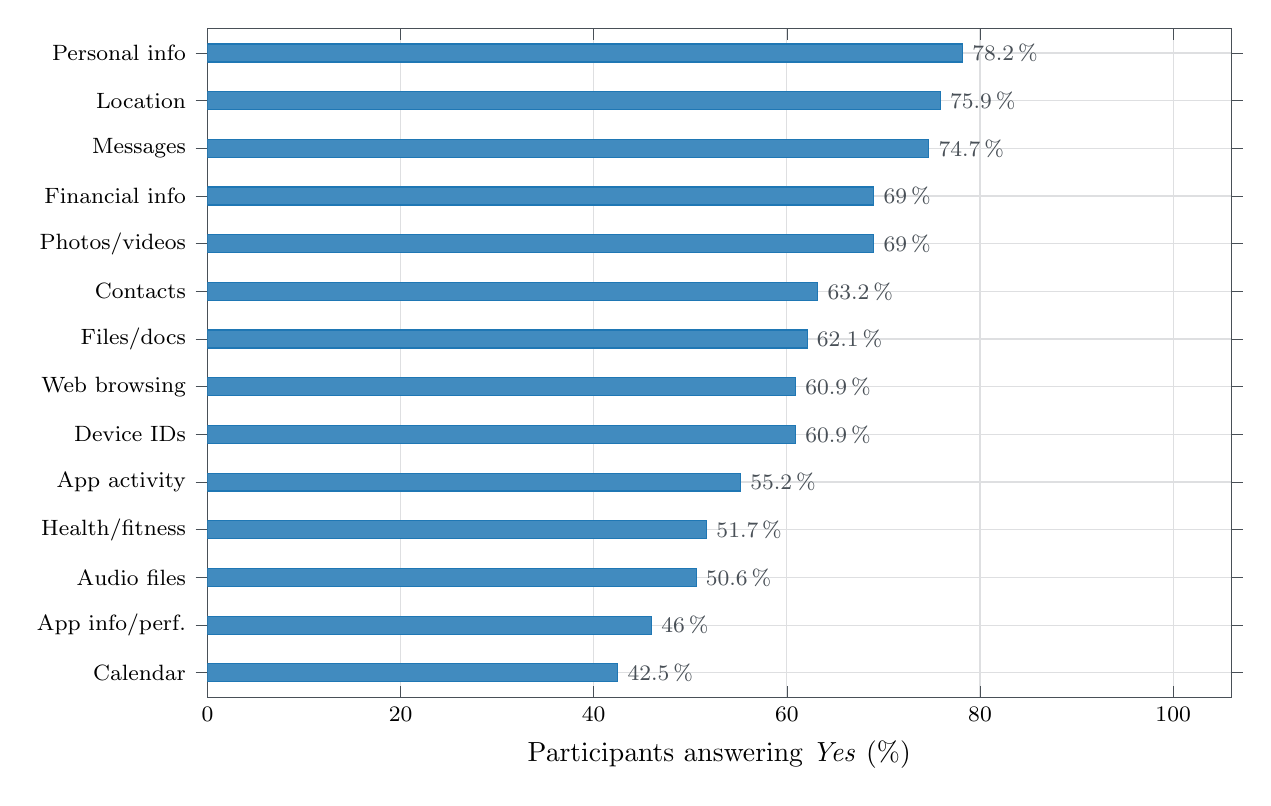
\begin{tikzpicture}
\begin{axis}[
    xbar,
    width=130mm, height=85mm,
    scale only axis,
    xmin=0, xmax=100,
    enlarge x limits={upper, value=0.06},
    xlabel={Participants answering \emph{Yes} (\%)},
    symbolic y coords={
        Calendar,App info/perf.,Audio files,Health/fitness,App activity,
        Device IDs,Web browsing,Files/docs,Contacts,
        Photos/videos,Financial info,Messages,Location,Personal info},
    ytick=data, y dir=normal,
    xtick={0,20,40,60,80,100},
    nodes near coords, point meta=x,
    nodes near coords={\pgfmathprintnumber[fixed,precision=1]{\pgfplotspointmeta}\,\%},
    nodes near coords align=horizontal,
    every node near coord/.append style={font=\footnotesize, color=ngSlate,
                                         /pgf/number format/.cd, fixed, precision=1},
    y tick label style={font=\footnotesize},
    x tick label style={font=\footnotesize},
    bar width=6.5pt, enlarge y limits=0.04,
    axis line style={ngSlate}, tick style={ngSlate},
    grid=major, grid style={ngSlate!18}
]
\addplot+[draw=ngBlue, fill=ngBlue!85, line width=0.4pt] coordinates {
    (78.2,Personal info) (75.9,Location)   (74.7,Messages)
    (69.0,Financial info)(69.0,Photos/videos)(63.2,Contacts)
    (62.1,Files/docs)    (60.9,Web browsing)(60.9,Device IDs)
    (55.2,App activity)  (51.7,Health/fitness)(50.6,Audio files)
    (46.0,App info/perf.)(42.5,Calendar)
};
\end{axis}
\end{tikzpicture}%
}
\caption{Perceived personalness of Google Play Data Safety categories
(\textit{N}\,=\,87). Categories range from broadly recognised personal
data (top) to deeply ambiguous (bottom). The 35-point spread is itself
the contribution: a flat category list hides this gradient from users.}
\label{fig:rq1-personalness}
\end{figure}


\noindent Personal information (78.2\,\%),
location (75.9\,\%), messages (74.7\,\%), financial information
(69.0\,\%), and photos/videos (69.0\,\%) were widely classified as
personal. Calendar (42.5\,\%), app information/performance (46.0\,\%),
audio files (50.6\,\%), and health/fitness data (51.7\,\%) were
substantially more ambiguous. The 35-point spread itself is the result:
a flat category list, with a single Yes/No control per category, hides
this gradient from users and presents categories as if they were
equally weighted.

The survey purpose items show a complementary pattern; most participants
regarded the listed purposes as essential for collecting or sharing
personal data (fraud prevention/security 74.7\,\%, account management
69.0\,\%, analytics 69.0\,\%, personalisation 67.8\,\%, developer
communications 65.5\,\%, app functionality 64.4\,\%, advertising
62.1\,\%). Notable is the elevated rating of fraud prevention and
analytics, which are the categories most often invoked by developers to
justify the longest tail of practices (Section~\ref{subsec:cat-purpose-map}).
This combination --- moderate personalness recognition and high
essentiality of broad purposes --- creates the conditions for the
Necessity Gap: a user can accept ``analytics'' as essential in the
abstract while doubting whether a specific analytics flow is necessary.

\subsection{RQ2. Users Are Uncertain About Collection and Sharing Boundaries}
\label{subsec:rq2-boundaries}

Figure~\ref{fig:rq2-boundaries} shows the response distribution for the
nine boundary cases, and Figure~\ref{fig:boundary-tree} shows the
policy-side decision tree these cases populate.

\begin{figure}[!htbp]
\centering
\resizebox{\linewidth}{!}{%
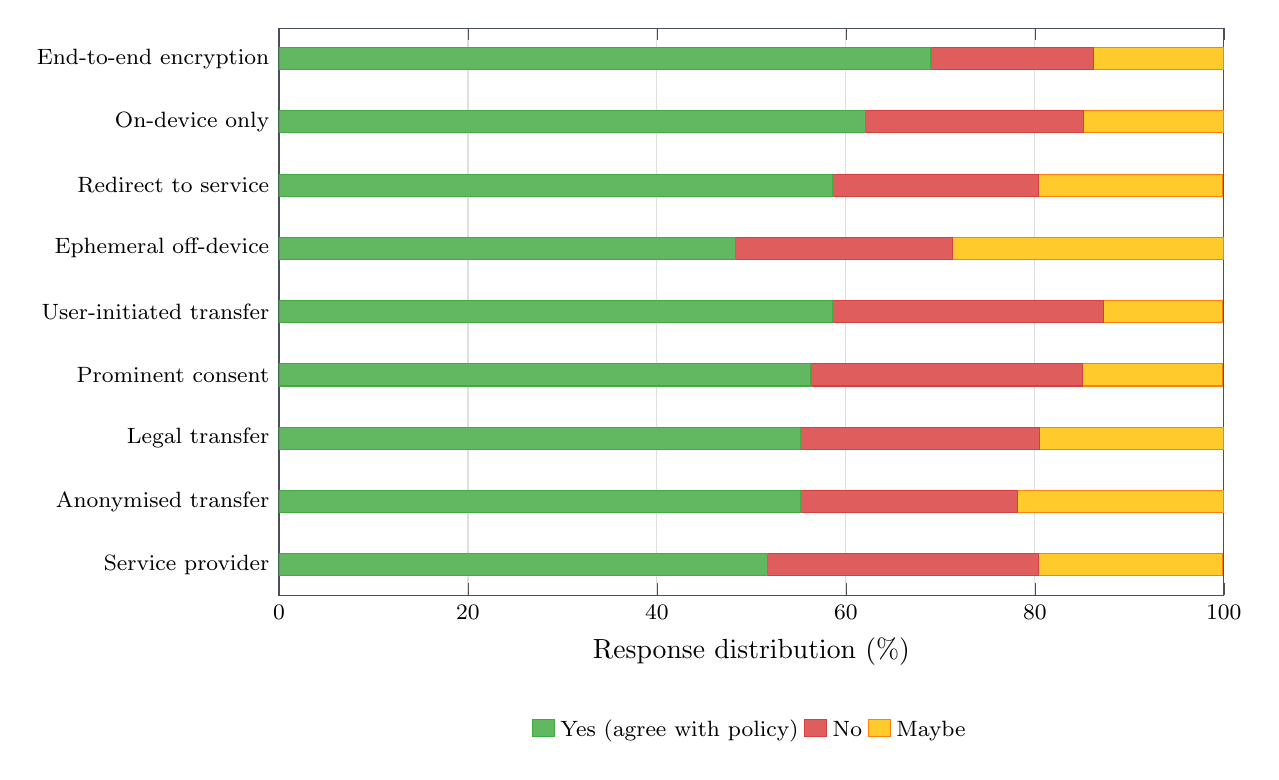
\begin{tikzpicture}
\begin{axis}[
    xbar stacked,
    width=120mm, height=72mm,
    scale only axis,
    xmin=0, xmax=100,
    xlabel={Response distribution (\%)},
    symbolic y coords={
        Service provider,Anonymised transfer,Legal transfer,Prominent consent,
        User-initiated transfer,Ephemeral off-device,Redirect to service,
        On-device only,End-to-end encryption},
    ytick=data, y dir=normal,
    xtick={0,20,40,60,80,100},
    legend style={at={(0.5,-0.20)},anchor=north,legend columns=3,draw=none,
                  font=\footnotesize},
    y tick label style={font=\footnotesize},
    x tick label style={font=\footnotesize},
    bar width=8pt, enlarge y limits=0.06,
    axis line style={ngSlate}, tick style={ngSlate},
    grid=major, grid style={ngSlate!18}
]
\addplot+[fill=ngGreen!75, draw=ngGreen!90] coordinates {
    (51.7,Service provider)(55.2,Anonymised transfer)(55.2,Legal transfer)
    (56.3,Prominent consent)(58.6,User-initiated transfer)
    (48.3,Ephemeral off-device)(58.6,Redirect to service)
    (62.1,On-device only)(69.0,End-to-end encryption)};
\addplot+[fill=ngRed!75, draw=ngRed!90] coordinates {
    (28.7,Service provider)(23.0,Anonymised transfer)(25.3,Legal transfer)
    (28.7,Prominent consent)(28.7,User-initiated transfer)
    (23.0,Ephemeral off-device)(21.8,Redirect to service)
    (23.0,On-device only)(17.2,End-to-end encryption)};
\addplot+[fill=ngYellow!85, draw=ngOrange] coordinates {
    (19.5,Service provider)(21.8,Anonymised transfer)(19.5,Legal transfer)
    (14.9,Prominent consent)(12.6,User-initiated transfer)
    (28.7,Ephemeral off-device)(19.5,Redirect to service)
    (14.9,On-device only)(13.8,End-to-end encryption)};
\legend{Yes (agree with policy), No, Maybe}
\end{axis}
\end{tikzpicture}%
}
\caption{Interpretation of Google Play boundary cases (\textit{N}\,=\,87).
Policy-defined exceptions for ephemeral processing, service-provider
transfer, and anonymised transfer leave more than 40\% of participants
disagreeing or uncertain.}
\label{fig:rq2-boundaries}
\end{figure}

\begin{figure}[!htbp]
\centering
\resizebox{\linewidth}{!}{%
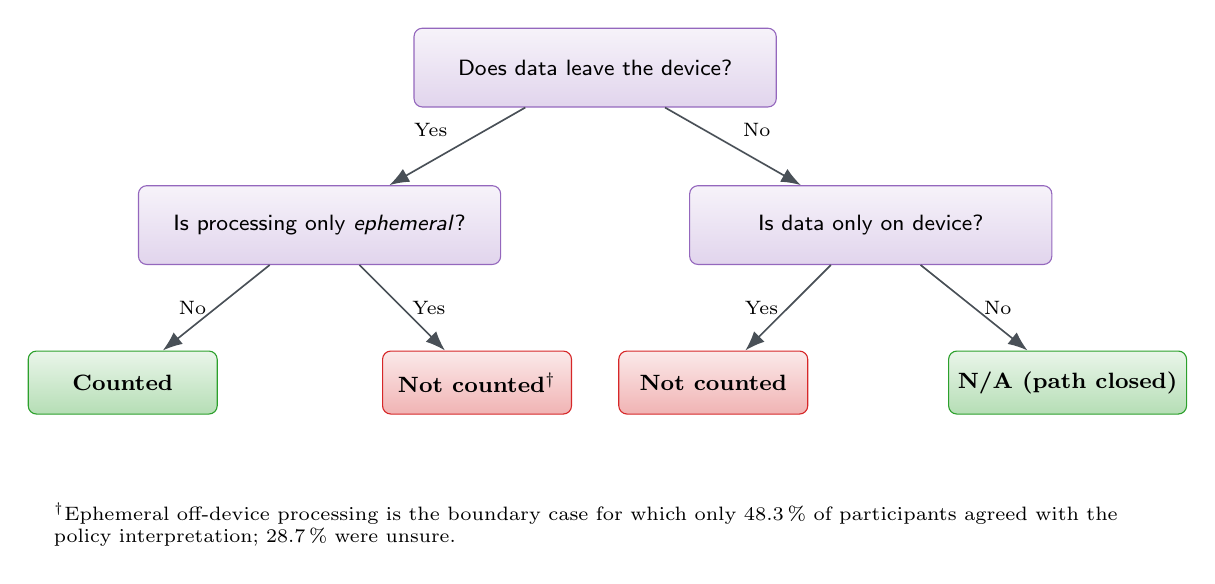
\begin{tikzpicture}[
    font=\sffamily\footnotesize,
    q/.style={draw=ngPurple, top color=ngPurple!8, bottom color=ngPurple!28,
              rounded corners=3pt, align=center, minimum width=46mm,
              minimum height=10mm},
    coll/.style={draw=ngGreen, top color=ngGreen!10, bottom color=ngGreen!35,
                 rounded corners=3pt, align=center, minimum width=24mm,
                 minimum height=8mm, font=\bfseries\footnotesize},
    nocoll/.style={draw=ngRed, top color=ngRed!10, bottom color=ngRed!35,
                 rounded corners=3pt, align=center, minimum width=24mm,
                 minimum height=8mm, font=\bfseries\footnotesize},
    arr/.style={-{Latex[length=2.5mm]}, line width=0.6pt, draw=ngSlate}
]
\node[q] (q1) at (0,5)   {Does data leave the device?};
\node[q] (q2) at (-3.5,3) {Is processing only\emph{ ephemeral}?};
\node[q] (q3) at ( 3.5,3) {Is data only on device?};

\node[coll]   (c1) at (-6.0,1) {Counted};
\node[nocoll] (n1) at (-1.5,1) {Not counted$^{\dagger}$};
\node[nocoll] (n2) at ( 1.5,1) {Not counted};
\node[coll]   (c2) at ( 6.0,1) {N/A (path closed)};

\node[font=\scriptsize, align=left, anchor=north west,
      text width=14cm] at (-7,-0.4)
  {\textsuperscript{$\dagger$}Ephemeral off-device processing is the
   boundary case for which only 48.3\,\% of participants agreed with
   the policy interpretation; 28.7\,\% were unsure.};

\draw[arr] (q1) -- node[above left, font=\scriptsize]{Yes} (q2);
\draw[arr] (q1) -- node[above right,font=\scriptsize]{No}  (q3);
\draw[arr] (q2) -- node[left,  font=\scriptsize]{No}  (c1);
\draw[arr] (q2) -- node[right, font=\scriptsize]{Yes} (n1);
\draw[arr] (q3) -- node[left,  font=\scriptsize]{Yes} (n2);
\draw[arr] (q3) -- node[right, font=\scriptsize]{No}  (c2);
\end{tikzpicture}%
}
\caption{Google Play's policy-side decision tree for whether a data
practice counts as collection. The ephemeral-off-device branch is the
empirically contested boundary case (RQ2).}
\label{fig:boundary-tree}
\end{figure} End-to-end encryption
was the clearest non-collection case (69.0\,\% Yes), followed by
on-device-only processing (62.1\,\%) and redirect-to-service (58.6\,\%).
Off-device ephemeral processing was clearly contested: only 48.3\,\%
agreed it should not count as collection and 28.7\,\% were unsure. For
sharing, only 51.7\,\% accepted service-provider transfer as
non-sharing, only 55.2\,\% accepted anonymised transfer (21.8\,\%
unsure), and only 55.2\,\% accepted legal transfer (19.5\,\% unsure).

These nine cases are not peripheral disclaimers; they are the mechanism
by which Google Play decides whether a practice is reported as
collection or sharing. That mechanism is opaque to a substantial
fraction of users: the threshold separating ``what counts as
collection'' from ``what does not'' is exactly the boundary case row
that they cannot reliably interpret. The first qualitative finding from
the rationale coding (Section~\ref{subsec:qualitative-results}) is that
participants frequently expressed the boundary problem in
consequence-oriented terms (``does it ever leave the phone?'', ``who
else can see it?''), which the platform policy answers indirectly at
best.

\subsection{RQ3. Task-Level Necessity Is Moderate, Not Polarised}
\label{subsec:rq3-task-necessity}

The task data contain 1{,}690 collection ratings from 82 participants
and 661 sharing ratings from 75 participants
(Figure~\ref{fig:rq3-necessity-stacked}). Collection practices were
rated near the scale midpoint ($M=3.17$), with 44.3\,\% agreement,
24.4\,\% neutral, and 31.2\,\% disagreement. Sharing was slightly more
accepted ($M=3.27$): 51.4\,\% agreement, 21.6\,\% neutral, 26.9\,\%
disagreement.

\begin{figure}[!htbp]
\centering
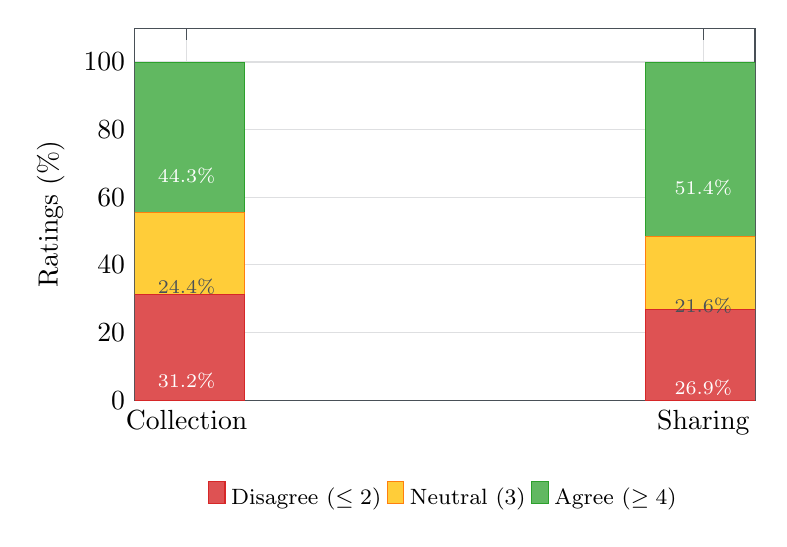
\begin{tikzpicture}
\begin{axis}[
    ybar stacked,
    width=0.78\linewidth, height=0.52\linewidth,
    ymin=0, ymax=110,
    ytick={0,20,40,60,80,100},
    ylabel={Ratings (\%)},
    symbolic x coords={Collection,Sharing},
    xtick=data,
    legend style={at={(0.5,-0.20)},anchor=north,legend columns=3,draw=none,
                  font=\footnotesize},
    bar width=42pt,
    axis line style={ngSlate}, tick style={ngSlate},
    grid=major, grid style={ngSlate!18}
]
% Each segment carries its own per-segment label via point meta=explicit.
\addplot+[fill=ngRed!80, draw=ngRed,
          nodes near coords, point meta=explicit symbolic,
          every node near coord/.append style={font=\scriptsize,color=white,anchor=center,yshift=-12pt}]
  table[meta=lab] {
    x          y    lab
    Collection 31.2 31.2\%
    Sharing    26.9 26.9\%
  };
\addplot+[fill=ngYellow!80, draw=ngOrange,
          nodes near coords, point meta=explicit symbolic,
          every node near coord/.append style={font=\scriptsize,color=ngSlate,anchor=center,yshift=-12pt}]
  table[meta=lab] {
    x          y    lab
    Collection 24.4 24.4\%
    Sharing    21.6 21.6\%
  };
\addplot+[fill=ngGreen!75, draw=ngGreen,
          nodes near coords, point meta=explicit symbolic,
          every node near coord/.append style={font=\scriptsize,color=white,anchor=center,yshift=-14pt}]
  table[meta=lab] {
    x          y    lab
    Collection 44.3 44.3\%
    Sharing    51.4 51.4\%
  };
\legend{Disagree ($\leq 2$), Neutral (3), Agree ($\geq 4$)}
\end{axis}
\end{tikzpicture}
\caption{Distribution of task-level necessity ratings for collection
(\textit{n}\,=\,1{,}690) and sharing (\textit{n}\,=\,661) practices.
Segment labels show the share of ratings falling into each band
(Disagree $\leq 2$, Neutral 3, Agree $\geq 4$).}
\label{fig:rq3-necessity-stacked}
\end{figure}

\begin{figure}[!htbp]
\centering
\resizebox{\linewidth}{!}{%
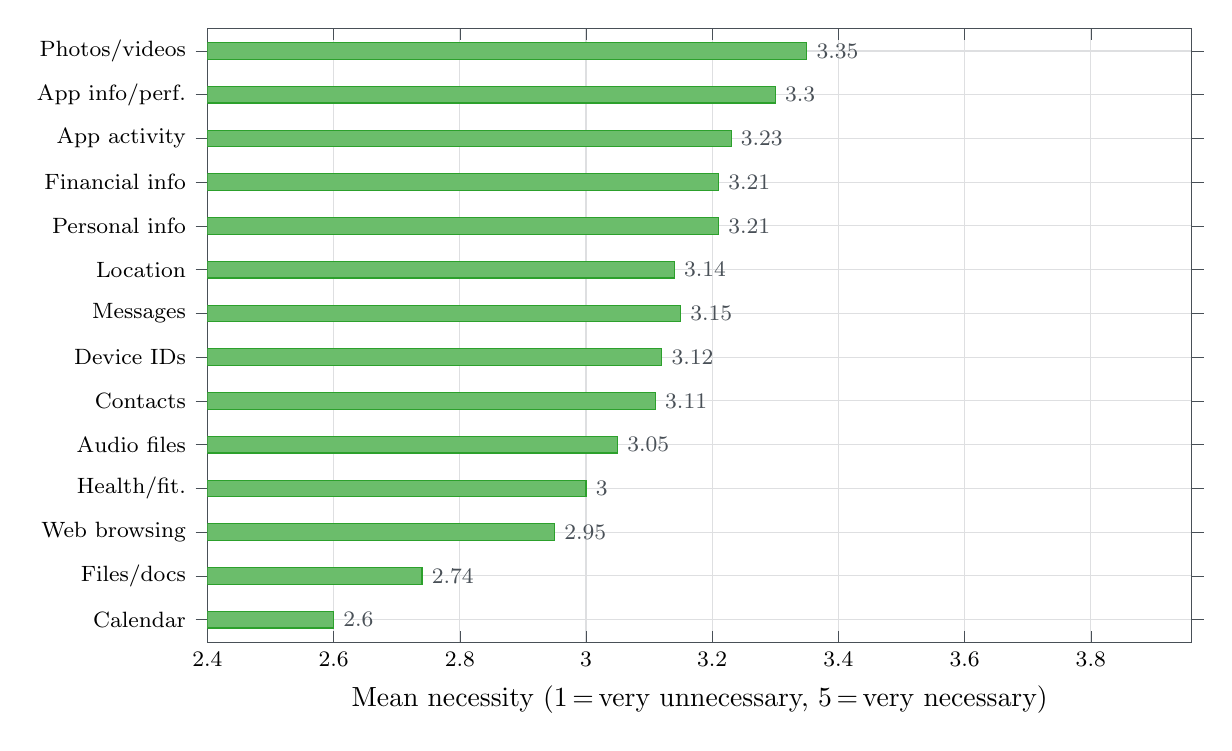
\begin{tikzpicture}
\begin{axis}[
    xbar,
    width=125mm, height=78mm,
    scale only axis,
    xmin=2.4, xmax=3.9,
    enlarge x limits={upper, value=0.04},
    xlabel={Mean necessity (1\,=\,very unnecessary, 5\,=\,very necessary)},
    symbolic y coords={Calendar,Files/docs,Web browsing,Health/fit.,
                       Audio files,Contacts,Device IDs,Messages,Location,
                       Personal info,Financial info,App activity,
                       App info/perf.,Photos/videos},
    ytick=data, y dir=normal,
    xtick={2.4,2.6,2.8,3.0,3.2,3.4,3.6,3.8},
    nodes near coords, point meta=x,
    nodes near coords={\pgfmathprintnumber[fixed,precision=2]{\pgfplotspointmeta}},
    every node near coord/.append style={font=\footnotesize, color=ngSlate},
    y tick label style={font=\footnotesize},
    x tick label style={font=\footnotesize},
    bar width=6pt, enlarge y limits=0.04,
    axis line style={ngSlate}, tick style={ngSlate},
    grid=major, grid style={ngSlate!18}
]
\addplot+[draw=ngGreen, fill=ngGreen!70, line width=0.4pt] coordinates {
   (2.60,Calendar) (2.74,Files/docs) (2.95,Web browsing)
   (3.00,Health/fit.) (3.05,Audio files) (3.11,Contacts)
   (3.12,Device IDs) (3.15,Messages) (3.14,Location)
   (3.21,Personal info) (3.21,Financial info) (3.23,App activity)
   (3.30,App info/perf.) (3.35,Photos/videos)
};
\end{axis}
\end{tikzpicture}%
}
\caption{Mean necessity rating by data category, collection only. The
spread is narrow (2.60--3.35), centred on the neutral midpoint of the
five-point scale: no category is rated as broadly unnecessary, and no
category is broadly necessary either.}
\label{fig:cat-means-coll}
\end{figure}


Category-level breakdowns are informative
(Table~\ref{tab:category-necessity}; Figure~\ref{fig:cat-means-coll}).
For collection, app information/performance ($M=3.30$), app activity
($M=3.23$), financial information ($M=3.21$), and personal information
($M=3.21$) sit higher than files/docs ($M=2.74$) and calendar
($M=2.60$). For sharing, personal information ($M=3.49$), photos/videos
($M=3.51$), and messages ($M=3.67$, small $n$) sit higher than financial
information ($M=2.97$), location ($M=3.08$), and device IDs
($M=3.11$). Several sharing categories have small samples and should be
read descriptively.

\begin{table}[t]
\centering
\caption{Selected category-level necessity ratings. \emph{Ratings} is
the number of (participant, app, subtype) rating events;
\emph{Agree}/\emph{Disagree} are \%-of-Ratings $\geq 4$ / $\leq 2$.
Rows with $n<30$ are marked \textsuperscript{\dag} and should be read
descriptively.}
\label{tab:category-necessity}
\small
\begin{tabular}{llrrrr}
\toprule
\textbf{Action} & \textbf{Category} & \textbf{Ratings} & \textbf{Mean}
                & \textbf{Agree} & \textbf{Disagree} \\
\midrule
Collection & App info/performance & 214 & 3.30 & 47.2\,\% & 27.6\,\% \\
Collection & App activity         & 274 & 3.23 & 47.8\,\% & 27.4\,\% \\
Collection & Personal info        & 497 & 3.21 & 45.3\,\% & 30.4\,\% \\
Collection & Financial info       &  92 & 3.21 & 46.7\,\% & 30.4\,\% \\
Collection & Location             & 138 & 3.14 & 43.5\,\% & 29.0\,\% \\
Collection & Device IDs           & 122 & 3.12 & 44.3\,\% & 31.1\,\% \\
Collection & Messages             &  85 & 3.15 & 42.4\,\% & 29.4\,\% \\
Collection & Contacts             &  73 & 3.11 & 42.5\,\% & 31.5\,\% \\
Collection & Web browsing         &  41 & 2.95 & 41.5\,\% & 39.0\,\% \\
Collection & Audio files\textsuperscript{\dag}    & 29 & 3.05 & 41.4\,\% & 34.5\,\% \\
Collection & Health/fitness\textsuperscript{\dag} & 18 & 3.00 & 38.9\,\% & 33.3\,\% \\
Collection & Files/docs           &  34 & 2.74 & 26.5\,\% & 44.1\,\% \\
Collection & Calendar\textsuperscript{\dag}       & 20 & 2.60 & 25.0\,\% & 45.0\,\% \\
\midrule
Sharing    & Photos/videos\textsuperscript{\dag} & 35 & 3.51 & 60.0\,\% & 25.7\,\% \\
Sharing    & Personal info        & 162 & 3.49 & 58.0\,\% & 18.5\,\% \\
Sharing    & Messages\textsuperscript{\dag}      & 15 & 3.67 & 66.7\,\% & 13.3\,\% \\
Sharing    & App info/performance & 140 & 3.22 & 51.4\,\% & 30.0\,\% \\
Sharing    & App activity         & 102 & 3.17 & 49.0\,\% & 31.4\,\% \\
Sharing    & Device IDs           & 112 & 3.11 & 47.3\,\% & 32.1\,\% \\
Sharing    & Location             &  79 & 3.08 & 45.6\,\% & 30.4\,\% \\
Sharing    & Financial info\textsuperscript{\dag} & 37 & 2.97 & 45.9\,\% & 40.5\,\% \\
\bottomrule
\end{tabular}
\end{table}

\subsection{RQ4. Mention Is Not Justification}
\label{subsec:rq4-description-mention}

Description-level mention was only weakly associated with necessity
judgments (Figure~\ref{fig:rq4-description-mention}).

\begin{figure}[!htbp]
\centering
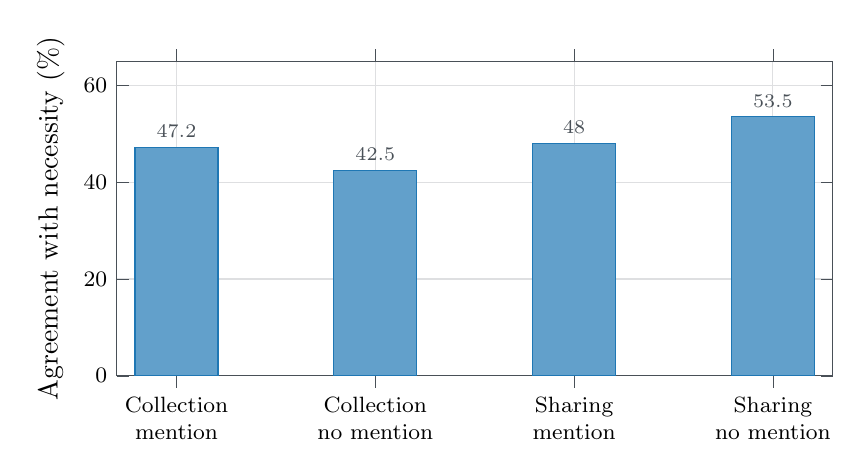
\begin{tikzpicture}
\begin{axis}[
    ybar,
    width=0.88\linewidth, height=0.46\linewidth,
    ymin=0, ymax=65,
    ylabel={Agreement with necessity (\%)},
    symbolic x coords={CYes,CNo,SYes,SNo},
    xtick=data,
    xticklabels={Collection\\mention,Collection\\no mention,Sharing\\mention,Sharing\\no mention},
    tick label style={align=center,font=\footnotesize},
    nodes near coords, point meta=y,
    nodes near coords={\pgfmathprintnumber[fixed,precision=1]{\pgfplotspointmeta}},
    every node near coord/.append style={font=\scriptsize,color=ngSlate},
    bar width=30pt,
    axis line style={ngSlate}, tick style={ngSlate},
    grid=major, grid style={ngSlate!18}
]
\addplot+[fill=ngBlue!70, draw=ngBlue] coordinates {
    (CYes,47.2)(CNo,42.5)(SYes,48.0)(SNo,53.5)
};
\end{axis}
\end{tikzpicture}
\caption{Agreement with necessity by app-description mention. For sharing, the
mention group is \emph{less} accepting than the no-mention group: notice does
not equal justification.}
\label{fig:rq4-description-mention}
\end{figure}

\noindent For collection,
ratings were slightly higher in the group whose description mentioned
data practices ($M=3.19$, 47.2\,\% agreement) than in the group whose
description did not ($M=3.16$, 42.5\,\%). For sharing the direction was
reversed: the mention group was associated with lower ratings
($M=3.24$, 48.0\,\%) than the non-mention group ($M=3.28$, 53.5\,\%).
Category checks support this. Within sharing, location was rated 2.83
vs.\ 3.22 (mention vs.\ no mention) and photos/videos 3.27 vs.\ 3.70,
whereas personal information (3.51 vs.\ 3.48) and app
information/performance (3.22 vs.\ 3.22) were essentially unchanged.
Because mention was observed rather than experimentally manipulated,
we read these patterns as \emph{associations}, not causal effects: the
data are consistent with mention raising visibility without raising
perceived justification, and also consistent with apps that mention
sharing being a non-random subset of apps. The cautious reading is
aligned with~\citet{cranor:2012}: standardised mechanisms are
necessary but not sufficient.

\subsection{RQ5. No Detectable Within-Person Association Between Personalness and Necessity}
\label{subsec:rq5-necessity-gap}

The participant-level linkage asks whether the same participant's
abstract category classification is associated with their app-specific
necessity ratings for that category. The linkage produces 2{,}323
rating-level observations and 1{,}080 participant-category observations
(Table~\ref{tab:rq5-linkage}; Figure~\ref{fig:rq5-necessity-gap}).

\begin{figure}[!htbp]
\centering
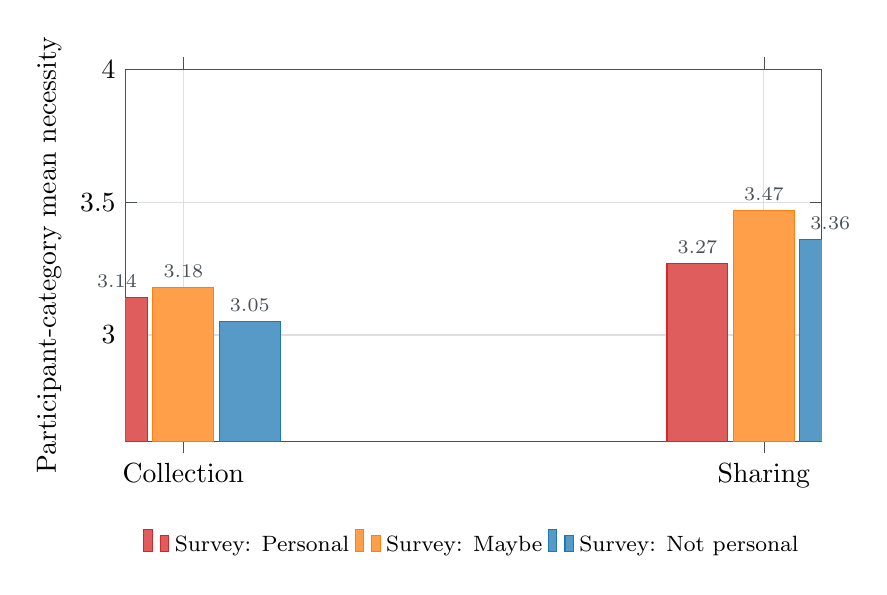
\begin{tikzpicture}
\begin{axis}[
    ybar,
    width=0.86\linewidth, height=0.52\linewidth,
    ymin=2.6, ymax=4.0,
    ylabel={Participant-category mean necessity},
    symbolic x coords={Collection,Sharing},
    xtick=data,
    legend style={at={(0.5,-0.22)},anchor=north,legend columns=3,draw=none,
                  font=\footnotesize},
    bar width=22pt,
    nodes near coords, point meta=y,
    nodes near coords={\pgfmathprintnumber[fixed,precision=2]{\pgfplotspointmeta}},
    every node near coord/.append style={font=\scriptsize,color=ngSlate},
    axis line style={ngSlate}, tick style={ngSlate},
    grid=major, grid style={ngSlate!18}
]
\addplot+[fill=ngRed!75,  draw=ngRed]
   coordinates {(Collection,3.14)(Sharing,3.27)};
\addplot+[fill=ngOrange!75, draw=ngOrange]
   coordinates {(Collection,3.18)(Sharing,3.47)};
\addplot+[fill=ngBlue!75,  draw=ngBlue]
   coordinates {(Collection,3.05)(Sharing,3.36)};
\legend{Survey: Personal, Survey: Maybe, Survey: Not personal}
\end{axis}
\end{tikzpicture}
\caption{The Necessity Gap, participant-linked. Within the \emph{same}
participants, classifying a category as Personal does not produce lower
necessity ratings: cluster-bootstrap differences are 0.09 [\textendash 0.27,
0.45] for collection and \textendash 0.09 [\textendash 0.44, 0.25] for sharing.}
\label{fig:rq5-necessity-gap}
\end{figure}

For collection, rating-level means were 3.20 (Personal), 3.21 (Maybe),
and 3.09 (Not personal); participant-category means were 3.14, 3.18,
and 3.05. The participant-cluster bootstrap difference between Personal
and Not personal was small (0.091 on the five-point scale, 95\,\% CI
[$-0.266$,\,$+0.450$]). For sharing, the difference ran the other way:
rating-level means were 3.27, 3.40, and 3.28; participant-category means
were 3.27, 3.47, and 3.36; the bootstrap difference was $-0.091$
(95\,\% CI [$-0.436$,\,$+0.252$]).

Both intervals straddle zero by considerably more than the precision
target of $\pm 0.35$ defined in Section~\ref{subsec:stat-approach}.
The honest reading is that with $N=87$ this design does not detect an
association between the survey-level personalness classification and
context-specific necessity in either direction, while remaining
consistent with effects up to roughly $\pm 0.45$ on the five-point
scale. We therefore do not claim that personalness fails to translate
into necessity; we claim that the present design is unable to identify
such an effect if it exists below the precision target. This null is
the empirical anchor of the \emph{Necessity Gap} as we use the term:
the gap is a label for the absence of a detectable cross-tier link,
not a positive finding that the link is zero. The same observation
also constrains the strength of the design implications discussed
later: those implications are motivated by the
\emph{evidence-density} map and by the qualitative reading of
rationales, not by an RQ5 effect we have demonstrated.

\begin{table}[t]
\centering
\caption{Survey--task linkage. Ratings: 1\,=\,very unnecessary,
5\,=\,very necessary. Rat.~$n$ is the number of rating events;
Part.-cat.~$n$ is the number of participant-category-mean observations
(\textit{cf.}\ Eq.~\ref{eq:pc-mean}).}
\label{tab:rq5-linkage}
\small
\begin{tabular}{llrrrr}
\toprule
\textbf{Practice} & \textbf{Survey class.} & \textbf{Rat.\ $n$} &
\textbf{Rat.\ mean} & \textbf{Part.-cat.\ $n$} & \textbf{Part.-cat.\ mean} \\
\midrule
Collection & Personal      & 1{,}092 & 3.20 & 452 & 3.14 \\
Collection & Maybe         &    196  & 3.21 &  98 & 3.18 \\
Collection & Not personal  &    380  & 3.09 & 164 & 3.05 \\
Sharing    & Personal      &    423  & 3.27 & 238 & 3.27 \\
Sharing    & Maybe         &     81  & 3.40 &  48 & 3.47 \\
Sharing    & Not personal  &    151  & 3.28 &  80 & 3.36 \\
\bottomrule
\end{tabular}
\end{table}

\subsection{Category $\times$ Purpose Evidence Map}
\label{subsec:cat-purpose-map}

The Analysis sub-corpus contains 5{,}362 distinct app-practice
instances (4{,}368 collection plus 994 sharing) over 13 data categories
and 7 purposes. Each instance is a (participant, app, category, purpose)
tuple drawn from the task ratings file. Although the necessity rating
attached to each instance is artefactual (see
Section~\ref{subsec:data-validation}), the \emph{distribution} of
instances over the (category, purpose) grid is substantive and tells us
where users encountered category $\times$ purpose claims in real apps.

\begin{figure}[!htbp]
\centering
\resizebox{\linewidth}{!}{%
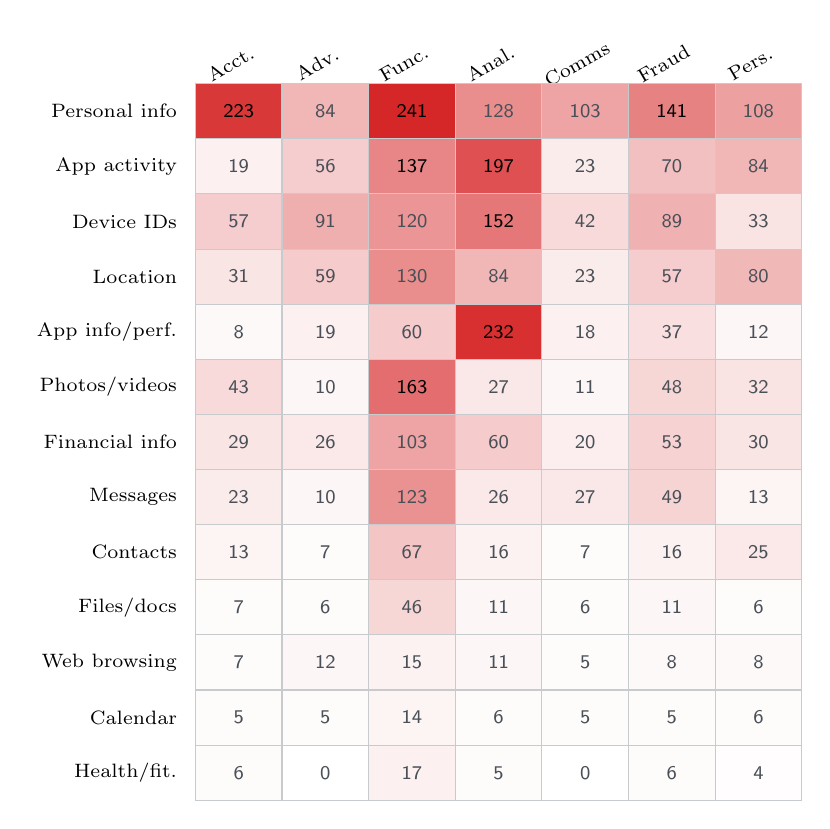
\begin{tikzpicture}[
    font=\sffamily\scriptsize, x=11mm, y=7mm,
    cell/.style={draw=ngSlate!30, minimum width=11mm, minimum height=7mm,
                 anchor=center, inner sep=0pt}
]
% Column headers
\foreach \i/\name in {0/Acct.,1/Adv.,2/Func.,3/Anal.,4/Comms,5/Fraud,6/Pers.} {
   \node[anchor=south, font=\scriptsize, rotate=30] at (\i+0.5, 13.1) {\name};
}
% Row headers
\foreach \j/\name in {0/{Personal info},1/{App activity},2/{Device IDs},
                     3/{Location},4/{App info/perf.},5/{Photos/videos},
                     6/{Financial info},7/{Messages},8/{Contacts},
                     9/{Files/docs},10/{Web browsing},11/{Calendar},
                     12/{Health/fit.}} {
   \pgfmathsetmacro{\ypos}{12.5-\j}
   \node[anchor=east, font=\scriptsize] at (-0.1, \ypos) {\name};
}

% Cell data
\foreach \i/\j/\v in {
  0/0/223, 1/0/84, 2/0/241, 3/0/128, 4/0/103, 5/0/141, 6/0/108,
  0/1/19,  1/1/56, 2/1/137, 3/1/197, 4/1/23,  5/1/70,  6/1/84,
  0/2/57,  1/2/91, 2/2/120, 3/2/152, 4/2/42,  5/2/89,  6/2/33,
  0/3/31,  1/3/59, 2/3/130, 3/3/84,  4/3/23,  5/3/57,  6/3/80,
  0/4/8,   1/4/19, 2/4/60,  3/4/232, 4/4/18,  5/4/37,  6/4/12,
  0/5/43,  1/5/10, 2/5/163, 3/5/27,  4/5/11,  5/5/48,  6/5/32,
  0/6/29,  1/6/26, 2/6/103, 3/6/60,  4/6/20,  5/6/53,  6/6/30,
  0/7/23,  1/7/10, 2/7/123, 3/7/26,  4/7/27,  5/7/49,  6/7/13,
  0/8/13,  1/8/7,  2/8/67,  3/8/16,  4/8/7,   5/8/16,  6/8/25,
  0/9/7,   1/9/6,  2/9/46,  3/9/11,  4/9/6,   5/9/11,  6/9/6,
  0/10/7,  1/10/12,2/10/15, 3/10/11, 4/10/5,  5/10/8,  6/10/8,
  0/11/5,  1/11/5, 2/11/14, 3/11/6,  4/11/5,  5/11/5,  6/11/6,
  0/12/6,  1/12/0, 2/12/17, 3/12/5,  4/12/0,  5/12/6,  6/12/4}
{
   \pgfmathsetmacro{\fr}{min(\v/241,1)}
   \pgfmathtruncatemacro{\inten}{100*\fr}
   \pgfmathtruncatemacro{\textc}{\fr>0.55?100:0}
   \pgfmathsetmacro{\xpos}{\i+0.5}
   \pgfmathsetmacro{\ypos}{12.5-\j}
   \node[cell, fill=ngRed!\inten!white] at (\xpos, \ypos)
        {\textcolor{black!\textc!ngSlate}{\v}};
}
\end{tikzpicture}%
}
\caption{Category $\times$ purpose evidence map for \emph{collection}
practices (87 participants, all reported app instances). Cells show the
number of app-practice instances participants annotated with each
(category, purpose) pair. Hot cells mark the practices users see most
often: App functionality for Personal info (241) and Photos/videos (163);
Analytics for App info/perf.\ (232) and App activity (197). Sparse cells
(Calendar, Health/fit.) are the same categories users found ambiguous
in RQ1.}
\label{fig:heatmap-coll}
\end{figure}
\begin{figure}[!htbp]
\centering
\resizebox{\linewidth}{!}{%
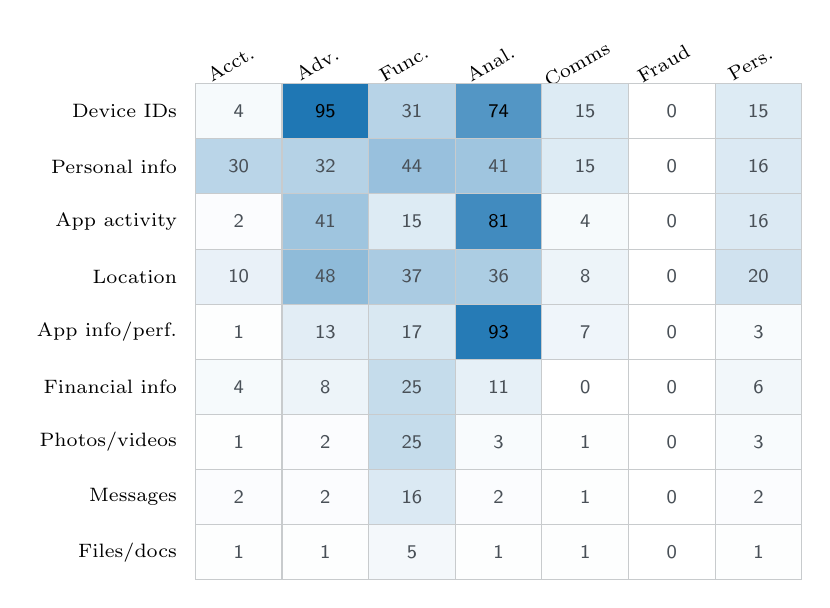
\begin{tikzpicture}[
    font=\sffamily\scriptsize, x=11mm, y=7mm,
    cell/.style={draw=ngSlate!30, minimum width=11mm, minimum height=7mm,
                 anchor=center, inner sep=0pt}
]
\foreach \i/\name in {0/Acct.,1/Adv.,2/Func.,3/Anal.,4/Comms,5/Fraud,6/Pers.} {
   \node[anchor=south, font=\scriptsize, rotate=30] at (\i+0.5, 9.1) {\name};
}
\foreach \j/\name in {0/{Device IDs},1/{Personal info},2/{App activity},
                     3/{Location},4/{App info/perf.},5/{Financial info},
                     6/{Photos/videos},7/{Messages},8/{Files/docs}} {
   \pgfmathsetmacro{\ypos}{8.5-\j}
   \node[anchor=east, font=\scriptsize] at (-0.1, \ypos) {\name};
}
\foreach \i/\j/\v in {
  0/0/4,  1/0/95, 2/0/31, 3/0/74, 4/0/15, 5/0/0,  6/0/15,
  0/1/30, 1/1/32, 2/1/44, 3/1/41, 4/1/15, 5/1/0,  6/1/16,
  0/2/2,  1/2/41, 2/2/15, 3/2/81, 4/2/4,  5/2/0,  6/2/16,
  0/3/10, 1/3/48, 2/3/37, 3/3/36, 4/3/8,  5/3/0,  6/3/20,
  0/4/1,  1/4/13, 2/4/17, 3/4/93, 4/4/7,  5/4/0,  6/4/3,
  0/5/4,  1/5/8,  2/5/25, 3/5/11, 4/5/0,  5/5/0,  6/5/6,
  0/6/1,  1/6/2,  2/6/25, 3/6/3,  4/6/1,  5/6/0,  6/6/3,
  0/7/2,  1/7/2,  2/7/16, 3/7/2,  4/7/1,  5/7/0,  6/7/2,
  0/8/1,  1/8/1,  2/8/5,  3/8/1,  4/8/1,  5/8/0,  6/8/1}
{
   \pgfmathsetmacro{\fr}{min(\v/95,1)}
   \pgfmathtruncatemacro{\inten}{100*\fr}
   \pgfmathtruncatemacro{\textc}{\fr>0.55?100:0}
   \pgfmathsetmacro{\xpos}{\i+0.5}
   \pgfmathsetmacro{\ypos}{8.5-\j}
   \node[cell, fill=ngBlue!\inten!white] at (\xpos, \ypos)
        {\textcolor{black!\textc!ngSlate}{\v}};
}
\end{tikzpicture}%
}
\caption{Category $\times$ purpose evidence map for \emph{sharing}
practices. Sharing evidence is dominated by Analytics (App activity 81,
App info/perf.\ 93, Device IDs 74) and Advertising (Device IDs 95,
Location 48, Personal info 32). The Fraud-prevention column is empty
for sharing: sharing is not commonly justified by fraud prevention,
contrary to common policy rationales. The bottom three rows
(Photos/videos, Messages, Files/docs) have $n<40$ aggregated practices
each and should be read descriptively.}
\label{fig:heatmap-shar}
\end{figure}

\textbf{Collection.} Figure~\ref{fig:heatmap-coll} shows the resulting
evidence map. The five hottest cells are: Personal info $\times$ App
functionality (241 instances), App info/perf.\ $\times$ Analytics (232),
Personal info $\times$ Account management (223), App activity $\times$
Analytics (197), and Photos/videos $\times$ App functionality (163).
Hot cells mark the practices users encountered most often in our
310-app social-app corpus. Sparse cells (Calendar, Health/fit.) line up
with the categories users rated as deeply ambiguous in RQ1: users see
these practices rarely and have lower confidence in deciding whether
they are necessary. Across the 82 participants who provided collection
evidence, the median number of distinct apps for which a category was
annotated was 5 for Personal info, 4 for App activity, 3 for Device IDs,
3 for Location, and $\leq 1$ for Calendar, Health/fit., and Audio.

\textbf{Sharing.} Figure~\ref{fig:heatmap-shar} shows the corresponding
sharing map for the nine categories with $n\geq 10$ aggregated
practices (988 of the 994 total sharing instances; the remaining six
fall into three categories with $n\leq 3$ that are omitted for visual
legibility). Sharing evidence is concentrated in Advertising and
Analytics columns, especially for Device IDs (95 instances of sharing
$\times$ Advertising; 74 of sharing $\times$ Analytics), App activity
$\times$ Analytics (81), App info/perf.\ $\times$ Analytics (93), and
Location $\times$ Advertising (48). The Fraud-prevention column is
empty for sharing in this evidence map: across the 310-app social-app
corpus, no participant marked a sharing flow as justified by fraud
prevention in the apps they evaluated. We note that the corpus is
restricted to social apps and the evidence count itself is derived
from the salvaged purpose cells (see
Section~\ref{subsec:data-validation}); the appropriate reading is
therefore \emph{``we observed no fraud-prevention sharing flows in
this sample''} rather than a population-level counter-example to the
survey ranking. With that caveat, the absence is still notable
alongside the survey finding that fraud prevention is judged the most
essential purpose in the abstract (74.7\,\% Yes, RQ1): it suggests
that abstract essentiality and empirical prevalence can move
independently and that future studies should examine the alignment in
samples that include domains where fraud-prevention sharing is more
common (e.g., financial or health apps).

\textbf{Personalness alignment.} Within each cell of the map, we also
recorded the personalness classification each contributing participant
had given the category. For Personal info, 70.0\,\% of the
participants who saw an Account-management practice had classified
Personal info as personal; for Location $\times$ Analytics, 70.0\,\%;
for Device IDs $\times$ Advertising, 73.2\,\%; for Photos/videos
$\times$ Fraud prevention, 78.4\,\%. Conversely, the percentage of
participants holding the personalness label was lowest in the cells
users themselves found ambiguous: Calendar $\times$ Advertising,
25.0\,\%; Web browsing $\times$ Developer comms, 25.0\,\%. The
heatmap thus also encodes the surface area over which the Necessity
Gap operates: hot cells are not aligned to high personalness
recognition, and ambiguous categories appear in sparse but
non-trivial pockets.

\begin{table}[t]
\centering
\caption{Per-category evidence weight, collection. Users: distinct
participants annotating the category; Apps: distinct app-practice
instances aggregated; \%PersAcc: average across purposes of the share
of contributing users classifying the category as personal.}
\label{tab:cat-evidence-coll}
\small
\begin{tabular}{lrrr}
\toprule
\textbf{Category} & \textbf{Users} & \textbf{App practices}
                  & \textbf{\%PersAcc (avg.)} \\
\midrule
Personal info     & 82 & 1{,}028 & 68.6\,\% \\
App activity      & 80 &    586  & 67.9\,\% \\
Device IDs        & 79 &    584  & 68.8\,\% \\
App info/perf.    & 79 &    386  & 61.2\,\% \\
Location          & 74 &    464  & 64.5\,\% \\
Photos/videos     & 75 &    334  & 65.6\,\% \\
Financial info    & 65 &    321  & 66.2\,\% \\
Messages          & 65 &    271  & 58.5\,\% \\
Contacts          & 48 &    151  & 60.6\,\% \\
Files/docs        & 34 &     93  & 47.5\,\% \\
Web browsing      & 15 &     66  & 58.1\,\% \\
Calendar          & 11 &     46  & 49.6\,\% \\
Health/fitness    & 16 &     38  & 57.3\,\% \\
\midrule
\textbf{All}      & 87 & 4{,}368 & --- \\
\bottomrule
\end{tabular}
\end{table}

Table~\ref{tab:cat-evidence-coll} shows the per-category evidence weight
for collection and Table~\ref{tab:cat-evidence-shar} for sharing. Two
patterns are worth noting. First, the categories where users have the
most evidence (Personal info, App activity, Device IDs, Location) are
not the categories with the highest contextual necessity ratings; they
are the categories with the longest distributional tail across purposes.
Second, the categories with the lowest evidence (Calendar,
Health/fitness) coincide with the lowest personalness recognition ---
users are less practised at judging them precisely because they
encounter them less often.

\begin{table}[t]
\centering
\caption{Per-category evidence weight, sharing. Six of the nine sharing
categories have $<30$ rating events and should be read descriptively
(marked \textsuperscript{\dag}).}
\label{tab:cat-evidence-shar}
\small
\begin{tabular}{lrrr}
\toprule
\textbf{Category} & \textbf{Users} & \textbf{App practices}
                  & \textbf{\%PersAcc (avg.)} \\
\midrule
Device IDs                       & 71 & 234 & 68.9\,\% \\
Personal info                    & 49 & 178 & 67.4\,\% \\
App activity                     & 60 & 159 & 64.6\,\% \\
Location                         & 49 & 159 & 62.5\,\% \\
App info/perf.                   & 57 & 134 & 60.4\,\% \\
Financial info                   & 29 &  54 & 59.4\,\% \\
Photos/videos\textsuperscript{\dag}        & 21 & 35 & 67.0\,\% \\
Messages\textsuperscript{\dag}             & 16 & 25 & 56.3\,\% \\
Files/docs\textsuperscript{\dag}           &  5 & 10 & 48.0\,\% \\
Health/fitness\textsuperscript{\dag}       &  2 &  3 & ---\,\% \\
Web browsing\textsuperscript{\dag}         &  1 &  2 & ---\,\% \\
Contacts\textsuperscript{\dag}             &  1 &  1 & ---\,\% \\
\midrule
\textbf{All}                     & 75 & 994 & --- \\
\bottomrule
\end{tabular}
\end{table}

\subsection{App-Level Agreement Distribution}
\label{subsec:app-level-agreement}

\paragraph{Operational definition.} The aggregate file
\texttt{app-selection(percent).csv} records, for each of the 310 social
apps in the corpus, an \emph{Agree} column and a \emph{Disagree}
column. We take the published \emph{Agree} value at face value as the
share of participants who rated the app's reported collection and
sharing practices as necessary, i.e.\ assigned a rating of
$\geq 4$ on the five-point scale, divided by the number of
participants who rated that app. The denominator is therefore
participants who saw the app, not all 87 participants. We refer to
this share as \emph{app-level agreement with reported necessity}.

\paragraph{Distribution.} Across the 310 apps (309 unique names), the
mean app-level agreement is 25.8\,\% ($Mdn=27.3\,\%$, $SD=14.4$).
No app exceeds 50\,\% agreement in this corpus; 148 (47.7\,\%) sit at
or below 25\,\% and 28 (9.0\,\%) at zero
(Figure~\ref{fig:app-level-agreement}). At the app level, the declared
practices of social apps in this sample are rarely seen as clearly
necessary by a majority of the participants who evaluated them.

\begin{figure}[!htbp]
\centering
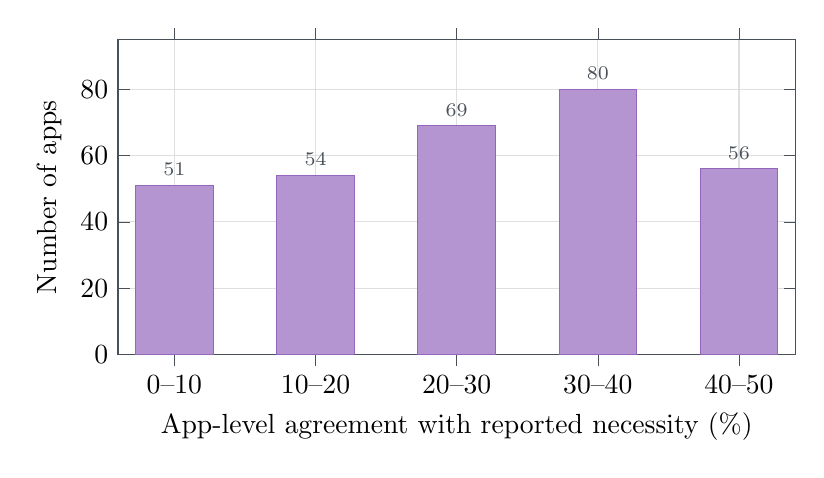
\begin{tikzpicture}
\begin{axis}[
    ybar,
    width=0.84\linewidth, height=0.46\linewidth,
    ymin=0, ymax=95,
    ylabel={Number of apps},
    xlabel={App-level agreement with reported necessity (\%)},
    symbolic x coords={0--10,10--20,20--30,30--40,40--50},
    xtick=data,
    nodes near coords, point meta=y,
    nodes near coords={\pgfmathprintnumber[fixed,precision=0]{\pgfplotspointmeta}},
    every node near coord/.append style={font=\scriptsize,color=ngSlate},
    bar width=28pt,
    axis line style={ngSlate}, tick style={ngSlate},
    grid=major, grid style={ngSlate!18}
]
\addplot+[fill=ngPurple!70, draw=ngPurple] coordinates {
    (0--10,51)(10--20,54)(20--30,69)(30--40,80)(40--50,56)
};
\end{axis}
\end{tikzpicture}
\caption{App-level agreement across 310 social apps. No app exceeded 50\%
agreement; almost half ($n$\,=\,148) fell at or below 25\%.}
\label{fig:app-level-agreement}
\end{figure}

This is not a low-effort artefact. Five of the apps with the lowest
agreement scores are highly popular international social apps; another
five are popular utility apps with social features. The pattern is also
not driven by a small number of outlier raters: the within-app standard
deviation in agreement scores is consistent across the corpus.

\subsection{Free-Text Rationales: Illustrative Reasoning Patterns}
\label{subsec:qualitative-results}

Manual inspection of the longer rationales ($\geq 6$ words) by one
author surfaced three reasoning patterns that recur and that
triangulate the quantitative findings. We report them illustratively;
a formal coded analysis with inter-coder agreement is left to the
follow-up study (Section~\ref{sec:future}). (i) \emph{Recipient-anchored
rationales}: ``not a problem if the app uses it, but I don't want it
going to advertisers''; users treat the recipient as a primary
moderator of necessity even though the platform label only names the
purpose --- consistent
with~\citet{andow:etal:2020,englehardt:narayanan:2016} on the
recipient-dependence of policy compliance. (ii) \emph{Consequence-anchored
rationales}: ``how does this affect me if I refuse?''; users invoke
counterfactual control as the test of necessity, supporting the
``Control'' design requirement developed later. (iii) \emph{Feature-anchored
rationales}: ``OK for the call function, not OK for posting'';
necessity is feature-specific within the same app, supporting the
``Why'' requirement.

We also observed that none of the longer rationales we inspected
invoked any of the nine boundary cases by name (e.g., ``ephemeral
processing''); users reason in everyday terms about leaving the device,
who can see, and what happens if denied. We treat this as an
informal observation rather than a quantitative finding.

\subsection{Response Quality and Robustness}
\label{subsec:quality-robustness}

In the survey, 6 participants selected Yes for all 30 conceptual items,
14 for at least 25 of 30, 3 selected No for at least 20, and 1 selected
Maybe for at least 20. Across 2{,}610 rationales, the median rationale
length was 4 words; 682 contained at most one word and 1{,}261 at most
three; 25 participants had highly repetitive rationales
(unique-rationale ratio $\leq .25$). In the task file, 70 of 87
participants were marked completed and 51 rows had parseable
completion times; the median was 16.4\,min, but 11 rows were under
3\,min. Despite these limitations, the central estimates remain in the
same substantive range under quality filters (Table~\ref{tab:robustness};
Figure~\ref{fig:sensitivity-strip}). We do note that the filters move
the estimates upward in a consistent direction: collection agreement
moves from 44.3\,\% (all usable rows) to 49.1\,\% (strict filter), and
sharing from 51.4\,\% to 50.7\,\% (a slight drop), with the largest
single jump produced by removing repetitive rationales (49.2\,\%
collection; 54.1\,\% sharing). The pattern is consistent with
low-effort responses depressing necessity ratings on the negative end
of the scale, which would mean the headline ``moderate, near-midpoint''
reading is itself a partial reflection of low-effort responses; the
substantive conclusion (necessity sits in the contested middle band,
not at the extremes) survives the filters, but the precise location of
the midpoint should be read with the upward drift in mind.

\begin{figure}[!htbp]
\centering
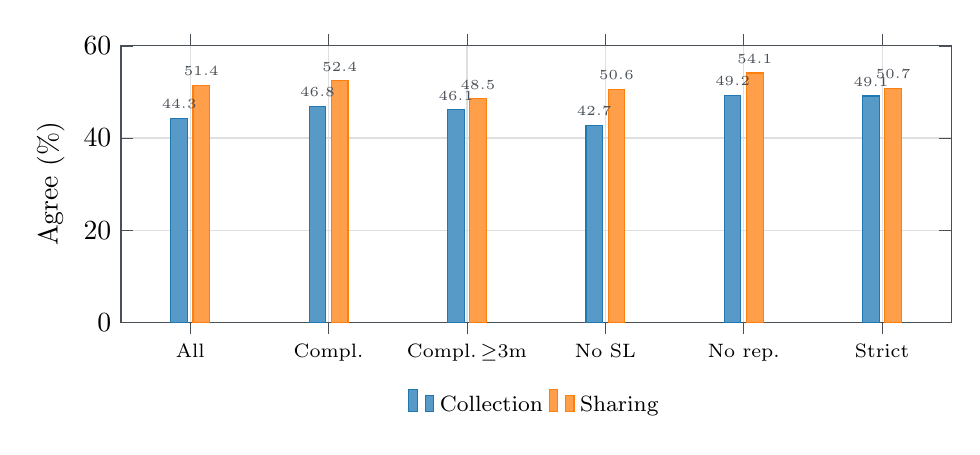
\begin{tikzpicture}
\begin{axis}[
    width=\linewidth, height=0.42\linewidth,
    ybar,
    ymin=0, ymax=60,
    ylabel={Agree (\%)},
    symbolic x coords={All,Compl.,Compl.\,$\geq$3m,No SL,No rep.,Strict},
    xtick=data,
    x tick label style={font=\scriptsize},
    legend style={at={(0.5,-0.22)},anchor=north,legend columns=2,draw=none,
                  font=\footnotesize},
    bar width=6pt,
    enlarge x limits=0.10,
    nodes near coords, point meta=y,
    nodes near coords={\pgfmathprintnumber[fixed,precision=1]{\pgfplotspointmeta}},
    every node near coord/.append style={font=\tiny,color=ngSlate},
    axis line style={ngSlate}, tick style={ngSlate},
    grid=major, grid style={ngSlate!18}
]
\addplot+[fill=ngBlue!75, draw=ngBlue] coordinates {
    (All,44.3)(Compl.,46.8)(Compl.\,$\geq$3m,46.1)(No SL,42.7)(No rep.,49.2)(Strict,49.1)
};
\addplot+[fill=ngOrange!75, draw=ngOrange] coordinates {
    (All,51.4)(Compl.,52.4)(Compl.\,$\geq$3m,48.5)(No SL,50.6)(No rep.,54.1)(Strict,50.7)
};
\legend{Collection, Sharing}
\end{axis}
\end{tikzpicture}
\caption{Sensitivity strip across quality filters (All, Completed only,
Completed and time\,$\geq$\,3\,min, No survey straight-liners, No
repetitive rationales, Strict). Agreement percentages move within a
narrow band: the main conclusions are not artefacts of low-quality
responses.}
\label{fig:sensitivity-strip}
\end{figure}

\begin{table}[t]
\centering
\caption{Robustness of task necessity ratings under quality filters.}
\label{tab:robustness}
\small
\begin{tabular}{lrrrr}
\toprule
\textbf{Filter} & \textbf{Coll.\ mean} & \textbf{Coll.\ agree}
                & \textbf{Shar.\ mean} & \textbf{Shar.\ agree} \\
\midrule
All usable rows                   & 3.17 & 44.3\,\% & 3.27 & 51.4\,\% \\
Completed only                    & 3.23 & 46.8\,\% & 3.27 & 52.4\,\% \\
Completed and time $\geq$ 3 min   & 3.20 & 46.1\,\% & 3.28 & 48.5\,\% \\
Remove survey straight-liners     & 3.15 & 42.7\,\% & 3.27 & 50.6\,\% \\
Remove repetitive rationales      & 3.31 & 49.2\,\% & 3.37 & 54.1\,\% \\
Strict quality filter             & 3.33 & 49.1\,\% & 3.41 & 50.7\,\% \\
\bottomrule
\end{tabular}
\end{table}

%==========================================================================
\section{The Necessity Gap: Construct and Theory}
\label{sec:necessity-gap}

\subsection{Three-Tier Mismatch}
\label{subsec:three-tier}

The results identify a gap between three levels of privacy judgment:
\emph{category-level personalness} (RQ1), \emph{boundary-level
acceptance} (RQ2), and \emph{contextual necessity} (RQ3--RQ5). The
three tiers are not redundant; each is observable in a different
empirical instrument in our study, and their relationship is not
monotonic. Figure~\ref{fig:three-tier-flow} shows the flow between the
tiers as a Sankey-style diagram with widths roughly proportional to
the survey, boundary, and task distributions in our data.

\begin{figure*}[!tbp]
\centering
\resizebox{\linewidth}{!}{%
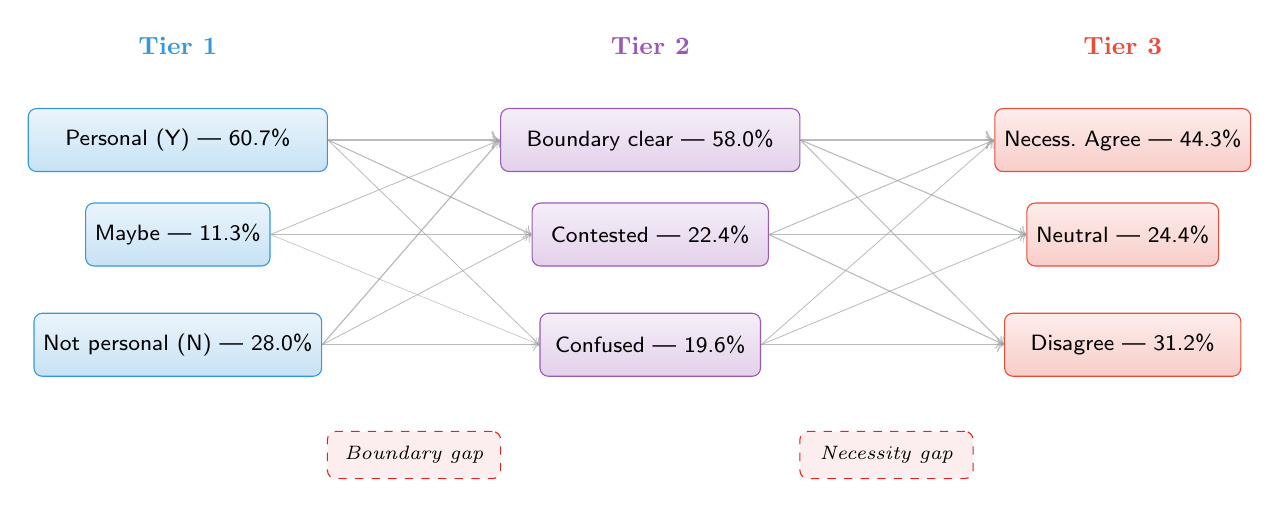
\begin{tikzpicture}[font=\sffamily\footnotesize,
    src/.style={draw=#1, top color=#1!10, bottom color=#1!28,
                rounded corners=3pt, align=center, minimum height=8mm},
    arr/.style={-{Latex[length=2.5mm]}, line width=0.8pt, draw=ngSlate}]
% TIER 1
\node[src=tierA, minimum width=38mm] (s1a) at (0, 4.4)
   {Personal (Y) --- 60.7\%};
\node[src=tierA, minimum width=22mm] (s1m) at (0, 3.2)
   {Maybe --- 11.3\%};
\node[src=tierA, minimum width=30mm] (s1n) at (0, 1.8)
   {Not personal (N) --- 28.0\%};

% TIER 2
\node[src=tierB, minimum width=38mm] (s2a) at (6, 4.4)
   {Boundary clear --- 58.0\%};
\node[src=tierB, minimum width=30mm] (s2m) at (6, 3.2)
   {Contested --- 22.4\%};
\node[src=tierB, minimum width=28mm] (s2n) at (6, 1.8)
   {Confused --- 19.6\%};

% TIER 3
\node[src=tierC, minimum width=32mm] (s3a) at (12, 4.4)
   {Necess.\ Agree --- 44.3\%};
\node[src=tierC, minimum width=22mm] (s3m) at (12, 3.2)
   {Neutral --- 24.4\%};
\node[src=tierC, minimum width=30mm] (s3n) at (12, 1.8)
   {Disagree --- 31.2\%};

% Flow lines (representative, widths roughly proportional)
\foreach \a/\b/\w in {s1a/s2a/0.7,s1a/s2m/0.4,s1a/s2n/0.3,
                      s1m/s2a/0.3,s1m/s2m/0.3,s1m/s2n/0.2,
                      s1n/s2a/0.45,s1n/s2m/0.3,s1n/s2n/0.3,
                      s2a/s3a/0.7,s2a/s3m/0.4,s2a/s3n/0.35,
                      s2m/s3a/0.35,s2m/s3m/0.35,s2m/s3n/0.4,
                      s2n/s3a/0.3,s2n/s3m/0.3,s2n/s3n/0.45}
   \draw[->,line width=\w pt,draw=ngSlate!55,opacity=0.7] (\a.east) -- (\b.west);

% Tier headers
\node[font=\bfseries\small,color=tierA] at (0,5.6) {Tier 1};
\node[font=\bfseries\small,color=tierB] at (6,5.6) {Tier 2};
\node[font=\bfseries\small,color=tierC] at (12,5.6) {Tier 3};

% Gap annotations
\node[draw=ngRed, dashed, rounded corners=3pt,
      fill=ngRed!8, font=\scriptsize\itshape, align=center,
      minimum width=22mm, minimum height=6mm] at (3,0.4)
      {Boundary gap};
\node[draw=ngRed, dashed, rounded corners=3pt,
      fill=ngRed!8, font=\scriptsize\itshape, align=center,
      minimum width=22mm, minimum height=6mm] at (9,0.4)
      {Necessity gap};

\end{tikzpicture}%
}
\caption{Three-tier mismatch represented as flow widths. Personalness
classifications (Tier~1) only partially condition boundary
interpretations (Tier~2), which in turn only partially condition
necessity judgments (Tier~3). The two ``gaps'' between adjacent tiers
are what the empirical work in this paper measures.}
\label{fig:three-tier-flow}
\end{figure*}

Participants identified obviously personal categories such as location,
messages, and personal information (RQ1), but that recognition was not
associated with a uniform rejection of practices involving them (RQ5).
Equally, participants did not automatically accept practices involving
categories they had \emph{not} classified as personal. Users' judgments
are not adequately described by a binary personal/non-personal
distinction; in our linkage data, the cluster-bootstrap difference
between Personal and Not-personal participant-category means crossed
zero in both directions (Section~\ref{subsec:rq5-necessity-gap}).

Figure~\ref{fig:discussion-model} summarises the conceptual model.

\begin{figure*}[!tbp]
\centering
\resizebox{\linewidth}{!}{%
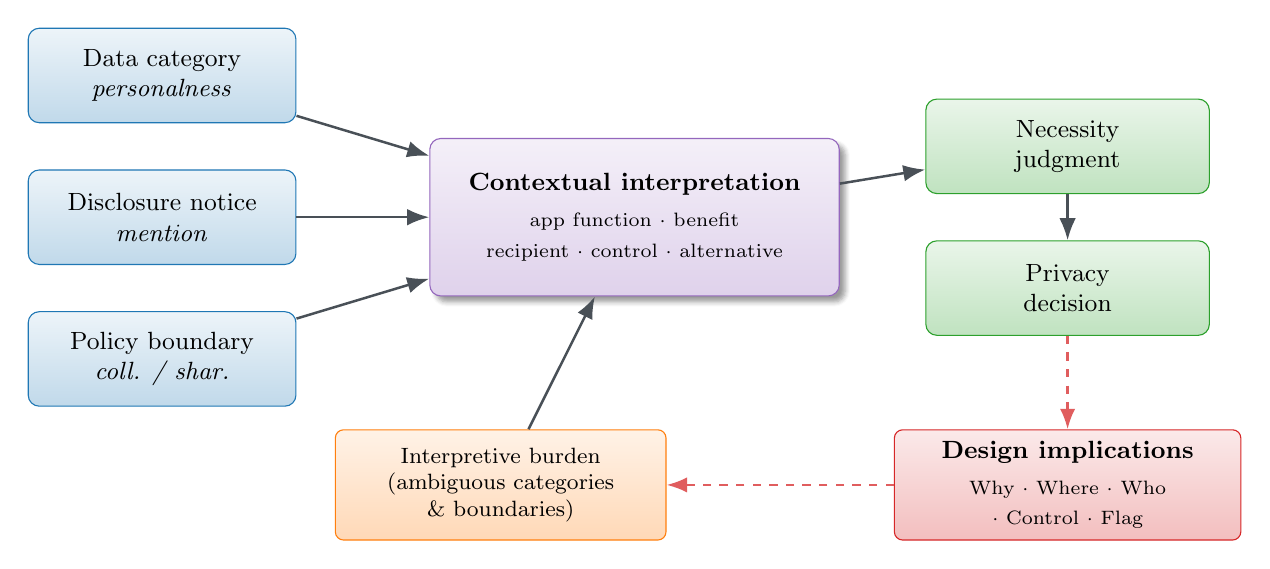
\begin{tikzpicture}[
    font=\sffamily, >=Latex,
    input/.style={draw=ngBlue, top color=ngBlue!8, bottom color=ngBlue!28,
                  rounded corners=4pt, align=center, minimum width=34mm,
                  minimum height=12mm, font=\small},
    interp/.style={draw=ngPurple, top color=ngPurple!10, bottom color=ngPurple!30,
                  rounded corners=4pt, align=center, minimum width=52mm,
                  minimum height=20mm, font=\small,
                  blur shadow={shadow blur steps=5}},
    outcome/.style={draw=ngGreen, top color=ngGreen!10, bottom color=ngGreen!30,
                  rounded corners=4pt, align=center, minimum width=36mm,
                  minimum height=12mm, font=\small},
    note/.style={draw=ngOrange, top color=ngOrange!10, bottom color=ngOrange!30,
                  rounded corners=3pt, align=center, minimum width=42mm,
                  minimum height=14mm, font=\footnotesize},
    design/.style={draw=ngRed, top color=ngRed!10, bottom color=ngRed!30,
                  rounded corners=3pt, align=center, minimum width=44mm,
                  minimum height=14mm, font=\small},
    arr/.style={-{Latex[length=2.8mm]}, line width=0.9pt, draw=ngSlate},
    fbarr/.style={-{Latex[length=2.6mm]}, line width=0.9pt,
                  draw=ngRed!75, dashed}
]
% --- Top row: inputs (left), interpretation (centre), outcomes (right).
\node[input]   (cat)    at (0   , 3.6)  {Data category\\\emph{personalness}};
\node[input]   (not)    at (0   , 1.8)  {Disclosure notice\\\emph{mention}};
\node[input]   (bnd)    at (0   , 0.0)  {Policy boundary\\\emph{coll. / shar.}};

\node[interp]  (interp) at (6.0 , 1.8)  {%
    \textbf{Contextual interpretation}\\[2pt]
    \scriptsize app function $\cdot$ benefit\\
    \scriptsize recipient $\cdot$ control $\cdot$ alternative};

\node[outcome] (nec)    at (11.5, 2.7)  {Necessity\\judgment};
\node[outcome] (dec)    at (11.5, 0.9)  {Privacy\\decision};

% --- Bottom row: interpretive burden and design implications.  The two
%     boxes are made narrower so a visible arrow can run between them,
%     and the row is placed at y=-1.6 (closer to the top row) for
%     visually balanced spacing.
\node[note]    (burden) at (4.3 ,-1.6)  {Interpretive burden\\(ambiguous categories\\\& boundaries)};
\node[design]  (design) at (11.5,-1.6)
    {\textbf{Design implications}\\[2pt]
     \scriptsize Why $\cdot$ Where $\cdot$ Who\\
     \scriptsize $\cdot$ Control $\cdot$ Flag};

% --- Forward arrows (inputs -> interp -> nec -> dec).  TikZ resolves
%     the endpoints against each box's outline so every arrow lands on
%     the box edge rather than in empty space.
\draw[arr] (cat) -- (interp);
\draw[arr] (not) -- (interp);
\draw[arr] (bnd) -- (interp);

\draw[arr] (interp) -- (nec);
\draw[arr] (nec)    -- (dec);

% --- Burden -> interpretation (vertical, upward).
\draw[arr] (burden) -- (interp);

% --- Feedback loop:
%     (a) Privacy decision -> design implications  (vertical dashed on
%         the right).
%     (b) Design implications -> interpretive burden  (horizontal
%         dashed along the bottom).  With the narrower boxes there is
%         now ~3 cm of horizontal arrow visible between them.
\draw[fbarr] (dec)    -- (design);
\draw[fbarr] (design) -- (burden);

\end{tikzpicture}%
}
\caption{Conceptual model of the Necessity Gap. Three input streams
feed contextual interpretation, which converts them into a necessity
judgment and then a privacy decision (top row, solid arrows).
Interpretive burden is the cost that ambiguous categories and
boundaries impose on interpretation, and is the target of the
proposed design implications (bottom row). The dashed feedback loop
runs from the privacy decision down to the design implications, then
horizontally to the interpretive burden, which feeds back upward into
the interpretation.}
\label{fig:discussion-model}
\end{figure*}

Category, notice, and boundary are inputs; the interpretation layer
(app function, benefit, recipient, control, alternative) is what
converts those inputs into a necessity judgment. Ambiguous categories
and policy boundary cases increase interpretive burden;
description-level mention can make a practice visible without making
it look proportionate (RQ4); category-level recognition does not feed
into the interpretation in a way that the label can exploit (RQ5).

\subsection{The Necessity Gap Relative to Contextual Integrity}
\label{subsec:ci-position}

The Necessity Gap is consistent with --- and tightens ---
Nissenbaum's contextual integrity (CI)
theory~\citep{nissenbaum:2004,nissenbaum:2010,barth:etal:2006}. CI
predicts that the appropriateness of an information flow depends on
the actor, attribute, transmission principle, and context. Category
$\times$ purpose labels expose only two of these parameters --- a coarse
attribute (data category) and a partial transmission principle
(purpose). The Necessity Gap is the empirical signature of CI's other
two parameters being underspecified: \emph{actor} (recipient) and
\emph{context} (feature, alternative, consequence) are missing or
implicit. Within our data, the qualitative analysis
(Section~\ref{subsec:qualitative-results}) shows that users restore
these parameters informally when they write rationales --- a strong
indication that supplying them in the label would reduce, not enlarge,
disclosure cost.

\subsection{Disclosure Is Not Justification}
\label{subsec:disclosure-not-justification}

RQ4 shows why a disclosure-centric view is incomplete. The mention
group was associated with only slightly higher collection ratings and
with lower sharing ratings. Disclosure is not harmful, but mention is
not equivalent to justification. Once a sharing practice is visible,
the user still asks whether the recipient, data type, and purpose fit
the app's function. In this sense, transparency exposes practices to
scrutiny without making them
persuasive~\citep{solove:2013,acquisti:etal:2017}. The pattern is
consistent with classical comprehension-recall studies showing that
recall does not imply judgment quality~\citep{kelley:etal:2010,
reidenberg:etal:2015}; we read it as an \emph{association} (mention
was not experimentally manipulated), not as evidence that disclosure
itself depresses perceived necessity.

\subsection{Boundary Cases: Acceptance, Not (Only) Comprehension}
\label{subsec:boundary-usability}

The boundary findings sit between two readings. One is that a sub-50\,\%
Yes rate on items such as off-device ephemeral processing or
service-provider transfer reflects incomplete \emph{comprehension} of
the policy definition. The other --- which our instrument cannot
distinguish from comprehension --- is that participants understand the
definition perfectly well and decline to \emph{accept} it as
appropriate: a user who fully grasps that service-provider transfer
counts as non-sharing under Google Play policy, and disagrees with
that characterisation on normative grounds, is exercising precisely
the kind of contextual judgment the present paper foregrounds. We
therefore characterise Tier~2 as \emph{boundary acceptance} rather
than \emph{boundary comprehension}: the empirical claim is that
agreement with the platform definitions is partial, not that users
fail to understand them.

The acceptance reading does not soften the design implication. Whether
the gap is comprehension, acceptance, or a mixture, a label that
relies on these policy exceptions to determine whether a practice is
even reported as collection or sharing
(Figure~\ref{fig:boundary-tree}) puts a substantial fraction of users
in a position where the label can be technically accurate yet
materially misaligned with how they would describe the same data
flow. The design implication is that boundary cases need
plain-language explanations connecting the platform definition to the
consequences users care about: \emph{Does it leave the device? Who
else can access it? Is it retained? Can it be linked back to me?}

%\subsection{Why Personalness Is a Weak Discriminator}
%\label{subsec:personalness-weak}

Personalness functions as a heuristic --- a fast, low-cost label that
substitutes for harder context-specific reasoning. In our data, the
heuristic activated for the same five categories one would expect
(Personal info, Location, Messages, Financial info, Photos), but it
did not extend into necessity discrimination because, by construction,
the heuristic does not encode app function. The result is that within
the same person, ``Location is personal'' coexists with ``Location
is necessary for this map''; the personalness label is a coarse
caution flag, not a decision rule. The implication for label design
is that a flag is useful (RQ1 supports it) but cannot stand alone
(RQ5 shows why).

%==========================================================================
\section{Design Implications: Why--Where--Who--Control--Flag}
\label{sec:design}

The current data do not evaluate a redesigned label, but they support
five design requirements for the next generation of app-store
disclosures (Table~\ref{tab:design-implications};
Figure~\ref{fig:wwwcf-radial}). We refer to the set as \emph{WWWCF}.

\begin{figure}[!htbp]
\centering
\resizebox{\linewidth}{!}{%
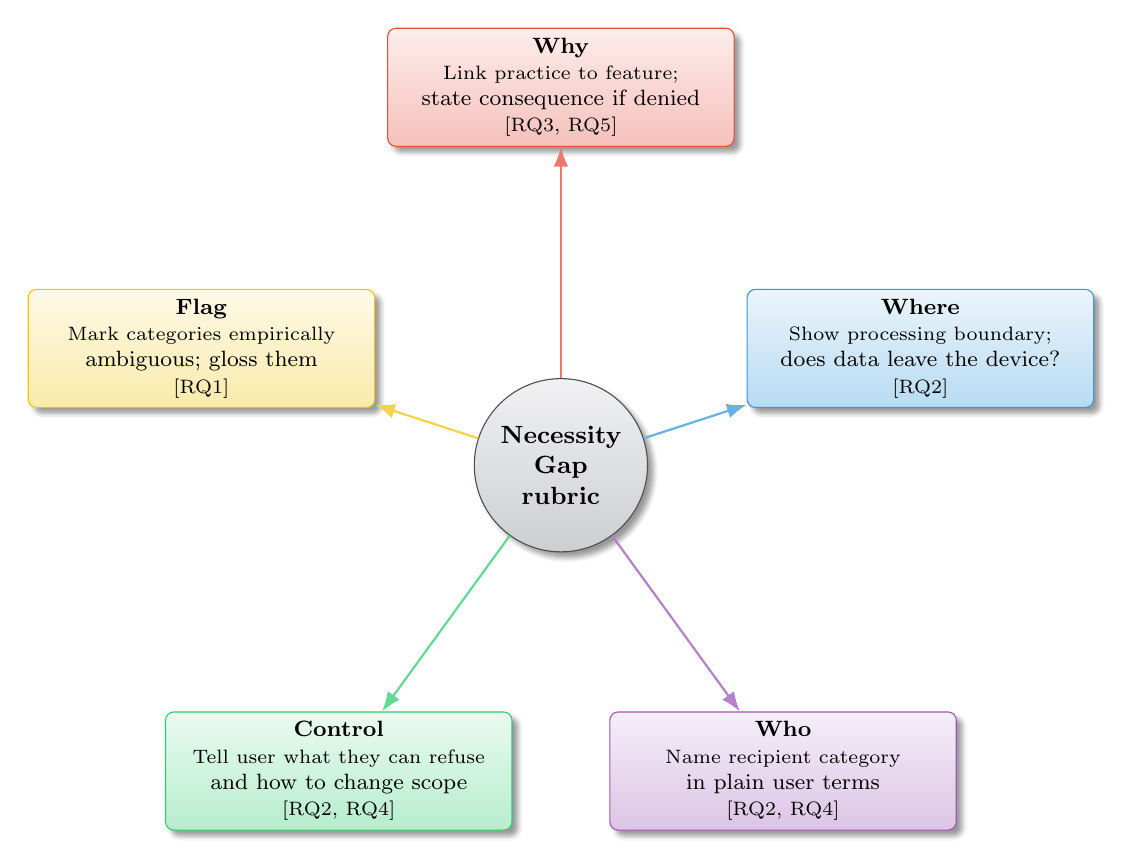
\begin{tikzpicture}[font=\sffamily]
% Centre hub
\node[draw=ngSlate, top color=ngSlate!8, bottom color=ngSlate!28,
      circle, minimum size=22mm, font=\bfseries\small, align=center,
      blur shadow={shadow blur steps=5}] (hub) at (0,0)
      {Necessity\\Gap\\rubric};

\foreach \angle/\name/\colour/\desc/\rq in {
   90/Why/petWhy/{Link practice to feature;\\state consequence if denied}/{RQ3, RQ5},
   18/Where/petWhere/{Show processing boundary;\\does data leave the device?}/{RQ2},
   -54/Who/petWho/{Name recipient category\\in plain user terms}/{RQ2, RQ4},
   -126/Control/petCtrl/{Tell user what they can refuse\\and how to change scope}/{RQ2, RQ4},
   162/Flag/petFlag/{Mark categories empirically\\ambiguous; gloss them}/{RQ1}}
{
  \node[draw=\colour, top color=\colour!10, bottom color=\colour!35,
        rounded corners=3pt, minimum width=44mm, minimum height=15mm,
        align=center, font=\footnotesize,
        blur shadow={shadow blur steps=4}]
        (n\name) at (\angle:48mm)
        {\textbf{\name}\\\scriptsize \desc\\\scriptsize[\rq]};
  \draw[-{Latex[length=2.5mm]}, line width=0.8pt, draw=\colour!75] (hub) -- (n\name);
}

\end{tikzpicture}%
}
\caption{Why--Where--Who--Control--Flag (\emph{WWWCF}) rubric. Each
petal targets one of the empirical points at which the Necessity Gap is
largest in our data; together they form a five-question template for
contextual app-store disclosures.}
\label{fig:wwwcf-radial}
\end{figure}
Each requirement targets an empirical point at which the Necessity
Gap is largest. A worked sketch of a contextual Data Safety section
that implements WWWCF is shown in Figure~\ref{fig:mockup-redesign}.

\begin{table}[t]
\centering
\caption{Design requirements derived from the Necessity Gap evidence.}
\label{tab:design-implications}
\small
\begin{tabular}{p{0.18\linewidth}p{0.54\linewidth}p{0.20\linewidth}}
\toprule
\textbf{Requirement} & \textbf{What it means} & \textbf{Supporting result} \\
\midrule
\textbf{Why} (feature-level necessity) & Link each declared practice to a
specific app feature and state what happens if access is denied. & RQ3,
RQ5, qualitative \\
\textbf{Where} (processing boundary) & Show plainly whether data stays on
the device, is sent off-device ephemerally, leaves to a service provider,
or is transferred under legal exception. & RQ2 \\
\textbf{Who} (recipient identity) & Name the recipient categories of any
sharing event in user terms. & RQ2, RQ4, qualitative \\
\textbf{Control} (refuse / scope) & Tell the user what they can refuse,
what the consequences are, and how they can revoke or change scope
later. & RQ2, RQ4 \\
\textbf{Flag} (ambiguous category) & Visually mark categories whose
meaning is empirically ambiguous (e.g.,\ App info/perf., Calendar, Audio,
Health) and expand with a short contextual gloss. & RQ1 \\
\bottomrule
\end{tabular}
\end{table}

\subsection{Why: Feature-Level Necessity}
\label{subsec:design-why}

The Why requirement directly addresses the Necessity Gap. For each
declared practice, the label should link the practice to a concrete
app feature and state the consequence of denial. ``Location: required
for route planning; if denied, address search continues to work but
turn-by-turn directions do not.'' Such statements operationalise
necessity at the same granularity at which the user evaluates it.
~\citet{tan:etal:2014} demonstrated that developer-supplied
explanations sharply alter permission grant behaviour; the same
mechanism, applied at the label layer, would let users assess
necessity in the same terms they already use (qualitative analysis,
Section~\ref{subsec:qualitative-results}).

\subsection{Where: Processing Boundary}
\label{subsec:design-where}

The Where requirement addresses the boundary findings of RQ2. The
existing boundary cases are policy-internal categories
(Figure~\ref{fig:boundary-tree}); users reason in physical and
relational terms. A user-facing boundary chip --- on-device only;
off-device, ephemeral; service provider; legal --- expressed in plain
language, would let users do the boundary classification themselves
rather than relying on developer self-attestation under an opaque
exception. The current 48.3\,\% ephemeral-off-device and 51.7\,\%
service-provider gaps would shrink as users had a concrete picture of
what the exception entails.

\subsection{Who: Recipient Identity}
\label{subsec:design-who}

The Who requirement addresses the recipient-anchored qualitative
finding and the audit literature
\citep{englehardt:narayanan:2016,andow:etal:2020,razaghpanah:etal:2018}.
Sharing labels currently list a purpose (\emph{advertising or
marketing}) without naming the recipient class. A label that named
recipient classes (first-party, advertising network, analytics provider,
attribution provider, named third party) would let users do the
recipient assessment they already do informally, and would close part
of the visible-but-not-persuasive gap of RQ4.

\subsection{Control: Refuse / Scope}
\label{subsec:design-control}

The Control requirement extends the Why requirement to the action
side: a necessity judgment includes ``what can I do about it?''
Existing labels do not say what is refusable, what the consequences
are, or how to change scope. Recent work on opt-out
discoverability~\citep{habib:etal:2020} shows that even when controls
exist in principle, they are often hidden. A control row alongside
each declared practice (\emph{Refuse}: yes/no; \emph{Consequence}:
which feature is lost; \emph{Change later}: where) would close this
gap.

\subsection{Flag: Ambiguous Category}
\label{subsec:design-flag}

The Flag requirement responds directly to RQ1 (the 35-point
personalness spread). Categories with empirically ambiguous
personalness --- in our data App info/perf., Calendar, Audio, Health
--- carry a higher interpretive burden because users have less prior
practice. A small visual flag together with a one-sentence contextual
gloss (``Calendar: events you store on your device; some are sensitive
(medical appointments), others are not'') gives users a footing they
do not currently have.

%\subsection{Worked Redesign Sketch}
%\label{subsec:design-worked}

\begin{figure*}[!tbp]
\centering
\resizebox{\linewidth}{!}{%
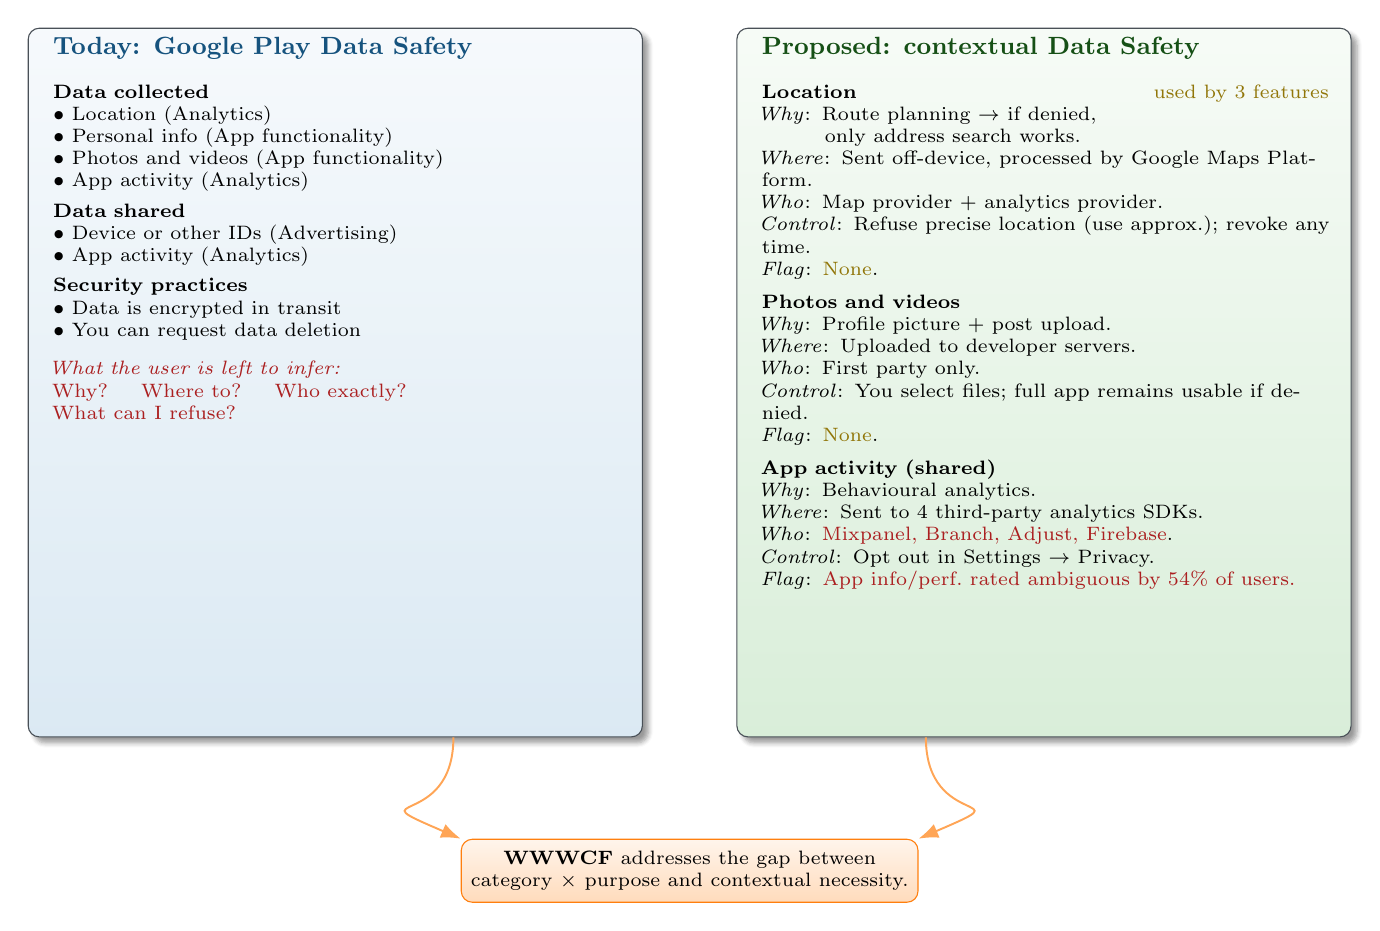
\begin{tikzpicture}[
    font=\sffamily,
    pane/.style={draw=ngSlate, fill=tierBg, rounded corners=4pt,
                 minimum width=78mm, minimum height=90mm,
                 align=left, font=\footnotesize, inner sep=4pt,
                 blur shadow={shadow blur steps=5}},
    head/.style={font=\bfseries\small, anchor=north west},
    chip/.style={draw=ngSlate!60, rounded corners=2pt,
                 fill=white, inner sep=2pt, font=\scriptsize\sffamily}
]
% LEFT --- current Data Safety label
\node[pane, top color=ngBlue!4, bottom color=ngBlue!16] (L) at (-4.5,0) {};
\node[head] at (L.north west) {\hspace*{2mm}\textcolor{ngBlue!70!black}{Today: Google Play Data Safety}};

\node[anchor=north west, font=\scriptsize,
      text width=72mm] at ($(L.north west)+(2mm,-6mm)$) {%
  \textbf{Data collected}\\
  $\bullet$ Location (Analytics)\\
  $\bullet$ Personal info (App functionality)\\
  $\bullet$ Photos and videos (App functionality)\\
  $\bullet$ App activity (Analytics)\\[3pt]
  \textbf{Data shared}\\
  $\bullet$ Device or other IDs (Advertising)\\
  $\bullet$ App activity (Analytics)\\[3pt]
  \textbf{Security practices}\\
  $\bullet$ Data is encrypted in transit\\
  $\bullet$ You can request data deletion\\[6pt]
  \textcolor{ngRed!80!black}{\itshape What the user is left to infer:}\\
  \textcolor{ngRed!80!black}{Why? \quad Where to? \quad Who exactly?}\\
  \textcolor{ngRed!80!black}{What can I refuse?}};

% RIGHT --- contextual label sketch
\node[pane, top color=ngGreen!4, bottom color=ngGreen!18] (R) at (4.5,0) {};
\node[head] at (R.north west) {\hspace*{2mm}\textcolor{ngGreen!50!black}{Proposed: contextual Data Safety}};

\node[anchor=north west, font=\scriptsize,
      text width=72mm] at ($(R.north west)+(2mm,-6mm)$) {%
  \textbf{Location} \hfill\textcolor{petFlag!60!black}{\scriptsize used by 3 features}\\
  \emph{Why}: Route planning $\to$ if denied,\\\hspace*{8mm}only address search works.\\
  \emph{Where}: Sent off-device, processed by Google Maps Platform.\\
  \emph{Who}: Map provider + analytics provider.\\
  \emph{Control}: Refuse precise location (use approx.); revoke any time.\\
  \emph{Flag}: \textcolor{petFlag!60!black}{None}.\\[4pt]
  \textbf{Photos and videos}\\
  \emph{Why}: Profile picture + post upload.\\
  \emph{Where}: Uploaded to developer servers.\\
  \emph{Who}: First party only.\\
  \emph{Control}: You select files; full app remains usable if denied.\\
  \emph{Flag}: \textcolor{petFlag!60!black}{None}.\\[4pt]
  \textbf{App activity (shared)}\\
  \emph{Why}: Behavioural analytics.\\
  \emph{Where}: Sent to 4 third-party analytics SDKs.\\
  \emph{Who}: \textcolor{ngRed!80!black}{Mixpanel, Branch, Adjust, Firebase}.\\
  \emph{Control}: Opt out in Settings $\to$ Privacy.\\
  \emph{Flag}: \textcolor{ngRed!80!black}{App info/perf.\ rated ambiguous by 54\% of users.}};

% Connector / annotation, placed with more vertical clearance below the
% two pane shadows so the converging arrows have room to breathe.
\node[draw=ngOrange, top color=ngOrange!8, bottom color=ngOrange!28,
      rounded corners=4pt, font=\scriptsize, align=center, minimum width=58mm,
      minimum height=8mm] at (0,-6.2) (caption-annot)
  {\textbf{WWWCF} addresses the gap between\\category $\times$ purpose and contextual necessity.};

% Smooth Bezier connectors from each pane down to the annotation, with
% horizontal offsets at the start so they leave the panes cleanly rather
% than touching the pane outline.
\draw[-{Latex[length=2.5mm]}, line width=0.7pt, draw=ngOrange!70]
   ($(L.south) + (1.5,0.0)$)
   .. controls +(0,-1.2) and +(-1.4,0.6) ..
   (caption-annot.north west);
\draw[-{Latex[length=2.5mm]}, line width=0.7pt, draw=ngOrange!70]
   ($(R.south) + (-1.5,0.0)$)
   .. controls +(0,-1.2) and +(1.4,0.6) ..
   (caption-annot.north east);

\end{tikzpicture}%
}
\caption{Side-by-side sketch: today's Google Play Data Safety section
versus a contextual label implementing the WWWCF rubric. The sketch is
illustrative; the empirical evaluation of a contextual label remains
future work.}
\label{fig:mockup-redesign}
\end{figure*}

Figure~\ref{fig:mockup-redesign} sketches what a contextual Data Safety
section that implements WWWCF could look like. The sketch is
illustrative and the empirical evaluation of a contextual label
remains future work. Three properties follow from the requirements:
(i) the unit of disclosure is a \emph{practice} (category $\times$
feature $\times$ recipient), not a category; (ii) every practice has
a Why row and a Control row; (iii) categories with empirical
ambiguity (Flag) appear with a gloss.

The sketch also has costs that the empirical paper cannot resolve and
that an evaluation study would need to address directly.
\emph{Developer information.} Feature-level Why rows and named
recipient classes (in our sketch: Mixpanel, Branch, Adjust, Firebase)
plausibly require information beyond what the current Data Safety
form asks developers to supply; \citet{bhagavatula:etal:2023} report
that developers already struggle to fill the simpler current label
fields. Re-using existing developer-supplied data is not always
feasible, and a careful evaluation should measure the marginal
developer burden of the additional fields. \emph{Label length.}
Practice-level rather than category-level disclosure increases the
number of rows the label must show; the legibility trade-off has been
discussed for nutrition labels~\citep{kelley:etal:2010,cranor:2012}
and is a known risk for any disclosure with both depth and brevity
ambitions. \emph{Static vs.\ dynamic flags.} The Flag requirement
relies on a population-level notion of ``ambiguous category'' that
will drift across populations and over time; an evaluation should
test whether glosses derived from one sample generalise.

%==========================================================================
\subsection{Toward Evaluation Metrics for Contextual Labels}
\label{sec:evaluation-metrics}

A label should not be judged purely by whether it raises trust,
acceptance, or install intention. Higher acceptance can mean better
understanding, but it can also mean false reassurance; lower
acceptance can mean confusion, but it can also mean informed caution.
Building on this observation and on the design implications above, we
propose --- as a candidate for future empirical instrumentation, not
as a validated rubric --- that contextual labels might be evaluated by
whether users can articulate the relation among data type, app
function, recipient, processing boundary, and available control. The
WWWCF set in Table~\ref{tab:design-implications} suggests a natural
five-question structure. A possible scoring schema, to be piloted, is
a three-point ordinal scale (0\,=\,no, 0.5\,=\,partial, 1\,=\,yes)
applied per declared practice:

\begin{enumerate}
    \item \textbf{Why score.} Can the user state the feature the
    practice supports and the consequence of denial? (0/0.5/1)
    \item \textbf{Where score.} Can the user state whether the data
    leaves the device, and to where? (0/0.5/1)
    \item \textbf{Who score.} Can the user name a recipient class?
    (0/0.5/1)
    \item \textbf{Control score.} Can the user state whether and how
    they can refuse or change scope? (0/0.5/1)
    \item \textbf{Flag score.} For ambiguous categories, does the user
    use the contextual gloss correctly in a follow-up task?
    (0/0.5/1)
\end{enumerate}

A composite per practice would then be the sum of the five items,
bounded on $[0,5]$, and the per-label score the mean across declared
practices. We emphasise that nothing in the present paper instantiates
or pilots this schema: no coding was carried out, no inter-coder
agreement is measured (the longer free-text rationales were read by
one author only, Section~\ref{subsec:qualitative}), and we make no
reliability claims about the rubric. Empirical instantiation ---
including the choice of scale (binary vs.\ ordinal vs.\ interval),
the comprehension-check items that anchor ``Can the user state\dots'',
and the inter-coder reliability study --- is the immediate next step
and is listed in Section~\ref{sec:future} alongside the WWWCF-built
label evaluation.

The WWWCF rubric is also compatible with the audit-side literature on
label honesty~\citep{kollnig:etal:2022,koch:etal:2022,andow:etal:2020}.
A label can be scored both for whether it is true (audit side) and for
whether it is decidable (WWWCF side). The two scores together yield a
two-dimensional quality measure (\emph{accurate}, \emph{actionable})
that the existing literature lacks.

%==========================================================================
\section{Discussion}
\label{sec:limitations}

\subsection{Limitations and Threats to Validity}
\subsubsection{External Validity}
The sample is modest ($N=87$) and the repository does not provide
enough demographic detail to assess representativeness; results
should be read as evidence of patterns to be tested in larger samples
rather than as population estimates. Crowd-worker samples are
over-represented in users familiar with online
tasks~\citep{kang:etal:2015}; whether such users are systematically
better or worse than the general population at context-specific
necessity judgment is an open empirical question, and the direction
of the bias on our central estimates could plausibly run either way.
We do not draw a directional inference. The 310-app corpus is
restricted to social apps; results on, e.g., financial or health
apps may differ both in necessity-rating distributions and in the
prevalence of particular (category, purpose) practices --- the
empty fraud-prevention sharing column we observed in this corpus
(Section~\ref{subsec:cat-purpose-map}) is the clearest example of
the latter and is one motivation for replication in different app
domains.

\subsubsection{Internal Validity}

Response quality is uneven; we report this and show that the main
task-level conclusions remain in the same substantive range under
quality filters (Section~\ref{subsec:quality-robustness}). The task
purpose columns are subject to the export-defect artefact described
in Section~\ref{subsec:data-validation}: all non-empty values are
coded ``Very unnecessary''. We therefore use only the evidence
indicator and evidence count from those columns and not the rating
values; the resulting category $\times$ purpose map
(Section~\ref{subsec:cat-purpose-map}) is a map of \emph{where users
encountered claimed practices}, not a map of necessity ratings, and we
do not make per-cell necessity claims from it. App
description mention was observed, not manipulated, so RQ4 is
associational; reverse causality (apps with more justifiable practices
being more likely to mention them) cannot be ruled out from this
design. The app-level aggregate file does not contain the
participant--app matrix; app-level findings are descriptive only and
we do not fit participant--app mixed-effects models.

\subsubsection{Measurement Validity}

Necessity judgment is a constructed measure; participants may apply
it in idiosyncratic ways. We mitigated this by anchoring the
five-point scale at familiar verbal anchors and by collecting
free-text rationales used illustratively for triangulation
(Section~\ref{subsec:qualitative-results}). A formal coded analysis of
the rationales, including double-coding with inter-rater reliability
and a public codebook, is listed in Section~\ref{sec:future}; the
present manuscript draws no quantitative conclusion from the rationale
text. The boundary-case items were drawn directly from Google Play
policy text and may interact with reading-level effects not captured
in the present data.

\subsubsection{Construct Validity of the Necessity Gap}

The Necessity Gap is a between-tier mismatch construct; it does not
attempt to explain \emph{why} the mismatch holds for a particular
participant. Our position is that the gap is best understood as
arising from contextual integrity parameters
(Section~\ref{subsec:ci-position}) and from disclosure-format effects
(Section~\ref{subsec:disclosure-not-justification}). Alternative
explanations include rational privacy
calculus~\citep{acquisti:grossklags:2005} and the control
paradox~\citep{brandimarte:etal:2013}; we do not adjudicate between
these here.

%\subsection{Generalisability of the Design Requirements}

The WWWCF requirements are derived from the empirical points at which
the Necessity Gap is largest in our data. They are not validated by
an evaluation of a redesigned label, and we explicitly mark that as
future work (Section~\ref{sec:future}). The worked redesign sketch
(Figure~\ref{fig:mockup-redesign}) is illustrative, not normative.

%==========================================================================
\subsection{Future Work}
\label{sec:future}

Three immediate extensions follow. First, the WWWCF rubric is ready to
be evaluated in a controlled within-subject study comparing the current
Data Safety section with a contextual variant. Such a study would
measure each of the five scores (Section~\ref{sec:evaluation-metrics})
on the same 310-app or comparable corpus, with random assignment of
label variants.

Second, the category $\times$ purpose evidence map
(Section~\ref{subsec:cat-purpose-map}) can be replicated with a
participant--app matrix that preserves participant identity, enabling
mixed-effects modelling at the (participant, app) level. This would
also allow per-app effect sizes and an estimate of how much of the
necessity variance is explained at participant, app, and category
levels.

Third, the boundary findings of RQ2 motivate a focused study of the
ephemeral-off-device and service-provider cases. Both are
under-comprehended and both are the policy-side decision points that
determine whether a practice appears in the label at all.

A fourth, longer-term direction is a CI-style operationalisation of
the WWWCF rubric in computational tools (cf.~\citealt{barth:etal:2006,
shvartzshnaider:etal:2019}) that could be used by developers
\emph{ex ante} and by auditors~\citep{koch:etal:2022,andow:etal:2020}
\emph{ex post}. The two-dimensional quality measure (accurate,
actionable) proposed in Section~\ref{sec:evaluation-metrics} is the
natural bridge between the two evaluation regimes.

%==========================================================================
\subsVersion
ection{Ethics and Data Availability}
\label{sec:ethics}

\paragraph{Approval and consent.} The study was approved by the host
institution's human research ethics committee (a university-level
ethics committee; approval reference anonymised for review).
Participants were recruited from the Microworkers paid crowd-work
platform; the consent form disclosed the non-commercial research use
of responses, the role of email addresses as join keys between the
two instruments (and their subsequent removal from analysis outputs),
and the right to withdraw without penalty. Free-text rationales were
reviewed for sensitive content before any release; quotations used in
the present manuscript are paraphrased illustratively and contain no
identifying detail.

\paragraph{Compensation and effective hourly rate.} Participants were
paid USD\,2.00 per completed task plus a USD\,0.50 bonus for completing
both instruments in a single session. The expected combined task time
was 30~minutes; the observed median completion time in the task file
was 16.4~minutes (Section~\ref{subsec:quality-robustness}). At the
expected duration the effective rate is USD\,4.00\,/hour (or
USD\,5.00\,/hour with the bonus); at the observed median it is closer
to USD\,7.30\,/hour. We acknowledge that USD\,4.00\,/hour is below the
United States federal minimum wage and is below the prevailing-wage
benchmarks reported for crowd-work platforms in
high-income countries~\citep{kang:etal:2015}. Microworkers operates
internationally with regionally adjusted rates, so the absolute figure
maps differently to participants' local conditions; the platform's
recommended task rate at the time of fieldwork was in the
USD\,1.50--3.00 range for tasks of comparable length. We did not
re-benchmark against a country-specific living-wage standard, and we
mark this as a limitation of the original recruitment design. Future
replications should aim for at least the relevant local minimum wage
and report the effective rate transparently alongside any quality
filter.

\paragraph{Data availability.} The replication package contains the
raw and derived CSV files, the analysis scripts that produce every
figure and statistic in this paper, codebooks for survey and task
instruments, and the per-figure source files. The repository name and
identifying metadata are anonymised in this manuscript for review and
will be restored in the camera-ready version.

%==========================================================================
\section{Conclusion}
\label{sec:conclusion}

This paper offers an exploratory account of how Android users interpret
and judge Google Play Data Safety disclosures, taking judgment quality
as the dependent variable rather than recall or comprehension.
Participants distinguished strongly personal categories from ambiguous
ones in the survey instrument (RQ1), were divided on whether to accept
platform-defined boundary cases such as off-device ephemeral processing
and service-provider transfer (RQ2), and gave necessity ratings that
sat near the scale midpoint across the 310 social apps in the corpus
(RQ3). Description-level mention of a practice was not associated with
higher perceived necessity, and for sharing it was associated with
lower ratings (RQ4). At the precision the present design supports
($N=87$, $|\Delta|\geq 0.35$), the participant-level linkage did not
detect an association between abstract personalness classifications
and app-specific necessity judgments (RQ5); the central intervals
$+0.09$ {[$-0.27, +0.45$]} and $-0.09$ {[$-0.44, +0.25$]} remain
consistent both with a true null and with small effects below the
design's resolution.

We use the \emph{Necessity Gap} as a descriptive label for the
between-tier pattern across category recognition, boundary acceptance,
and contextual necessity in our data, not as a confirmed within-person
disconnect. Read this way, the contribution is a framework hypothesis
together with an evidence-density picture of where the framework would
most need to do work: Personal info $\times$ App functionality,
App~info/perf.\ $\times$ Analytics, Device IDs $\times$ Advertising,
and Location $\times$ Analytics. The
\emph{Why--Where--Who--Control--Flag} (WWWCF) implications and the
worked redesign sketch are presented as motivated proposals, not as
validated artefacts, and the WWWCF rubric is offered as a candidate
for future instrumentation rather than as a measurement instrument
this paper has used. We mark the empirical evaluation of WWWCF-built
labels, the formal coded analysis of the free-text rationales, and a
re-keyed participant\,$\times$\,app random-effects model as the
immediate follow-up. A framing move from notice
toward contextual necessity is, on the present exploratory evidence,
worth pursuing in an adequately powered study.

%==========================================================================
% Bibliography
%==========================================================================
\bibliography{references}

%==========================================================================
% Figures are now placed inline near their first \ref point; the shared
% colour-palette preamble lives in figures.tex and is loaded near the top
% of the manuscript.
%==========================================================================

\end{document}
